\documentclass[../main.tex]{subfiles}

\begin{document}
    \subsubsection*{Uncertainties}
        Every following uncertainty was calculated using this formula
        \[u:=\fdef{\fdef{\sqrt{\sum_{i\in\text{Def}(x)}\diff{f}{u(x_i)}{x}{}}}{x\in\text{Def}{f}}}{f\in C^(\R^d,\R)}.\]
		        
        
    \subsection{Isentropric Exponent}
        \subsubsection*{Measurement according to Rüchhardt and Flammersfed}
            The measurements as described in \ref{sec:RuchhartFlammersfeld} yielded the following results for the isentropic exponent:

            \begin{table}[H]
                \centering
                \begin{tabular}{c|c|c}
                    \textbf{Gas} & \textbf{Oscillation period in s} & \textbf{Isentropic exponent}\\
                    \hline
                    $\text{Ar}$ & $0.9040(31)$ & $1.808$\\
                    $\text{CO}_2$ & $1.2050(31)$ & $1.406$\\
                    $\text{N}_2$ & $1.266(67)$ & $0.921$\\
                \end{tabular}
                \caption{isentropic exponents for different gases. The oscillation period refers to the oscillation period of the small metal cylinder. No Uncertainties are given because of their neglible size}
                \label{fig:KappaRuchhardtFlammersfeld}
            \end{table}

            \noindent Compared to the literature values of $\kappa_{\text{Ar}}=1.648$, $\kappa_{\text{N}_2}=1.401$, $\kappa_{\text{CO}_2}=1.293$, the obtain values are close but not compatible \cite[p.258]{skript}. One cause for this are the small used uncertainties. Thus, there may be some larger uncertainties yet to be accounted for.

        \subsubsection*{Clément and Desormes}
            Following the experiment described by Clément and Desormes \ref{sec:ClementDesormes}, we obtained the values for $\kappa$ depicted below:
            
            \begin{table}[H]
                \centering
                \begin{tabular}{c|cc|c}
                    \textbf{Gas} & \textbf{Height $h_1$ in cm} & \textbf{Height $h_1$ in cm} & \textbf{Isentropic exponent}\\
                    \hline
                    $\text{Ar}$ & $9.46(30)$ & $7.16(30)$ & $4.12(46)$\\
                    $\text{CO}_2$ & $10.26(30)$ & $7.26(30)$ & $3.42(18)$\\
                    $\text{N}_2$ & $9.86(30)$ & $7.29(30)$ & $3.84(32)$\\
                \end{tabular}
                \caption{isentropic exponents for different gases. $h_1$ and $h_3$ are the heights of the water pillar before and after the pressure release of the gas}
            \end{table}
            
            These measurements for $\kappa$ are almoust twice as much as the literature values or the ones in \ref{fig:KappaRuchhardtFlammersfeld}. One possible explanation is during the experiment, small air bubbles formed inside the water pillars, which might have rendered the formula connection $h_1,h_3$ and pressure differences inaccurate.

    \subsection{Degrees of freedom}
        For the analysis of the degrees of freedom we first need to consider noise. We also need to deal with an unknown uncertainty introduced by the microphon quality and the computers hardware and software algorithms. 
    \subsection*{Background noise}
        Before we start with the analysis of the data, we have to consider the background noise. We measured the background noise for the first measurement and obtained the following results:
        \begin{table}[H]
	\centering
	\begin{tabular}{ccccc}
		$\nu$ & c & C(c) & $\kappa$ & f\\
		\hline
		13.18(50) & 26.37(264) & 26.26(263) & 0.01(00) & -2.02(-02)	\\
		139.16(50) & 139.16(1392) & 138.99(139) & 0.34(003) & -3.04(-03)	\\
		269.53(50) & 179.69(1797) & 179.53(1795) & 0.57(006) & -4.65(-046)	\\
		404.3(50) & 202.15(2021) & 202.0(202) & 0.72(007) & -7.17(-072)	\\
		536.13(50) & 214.45(2145) & 214.32(2143) & 0.81(008) & -10.61(-106)	\\
		672.36(50) & 224.12(2241) & 224.0(224) & 0.89(009) & -17.58(-176)	\\
		805.66(50) & 230.19(2302) & 230.07(2301) & 0.93(009) & -30.72(-307)	\\
		940.43(50) & 235.11(2351) & 235.0(235) & 0.98(01) & -80.9(-809)	\\
		472.6(4726) & 181.4(1814) & 181.27(1813) & 0.66(007) & -19.59(-196)	\\
	\end{tabular}
\end{table}
        These we will then consider when choosing the peaks in the following analysis to not mistake them for false ones. 

    \subsection*{Analysis of first measure}
        We start analysing from high to low temperature. We will present the graphs and tables each. 
        
        \subsubsection*{73 degrees}
            \begin{figure}[H]
	\centering
	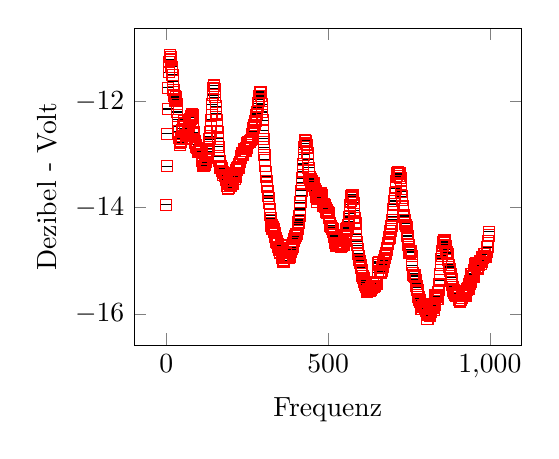
\begin{tikzpicture}
		\pgfplotsset{width=6.5cm,compat=1.3,legend style={font=\footnotesize}}
		\begin{axis}[xlabel={Frequenz},ylabel={Dezibel - Volt},legend cell align=left,legend pos=north west]
		\addplot+[only marks,color=red,mark=square,error bars/.cd,x dir=both,x explicit,y dir=both,y explicit,error bar style={color=black}] table[x=X,y=Y,x error=xerror,y error=yerror,row sep=\\]{			X	Y	xerror	yerror	\\			0.0	-13.944471	0	0	\\			1.464844	-13.218628	0	0	\\			2.929687	-12.60769	0	0	\\			4.394531	-12.141175	0	0	\\			5.859375	-11.741029	0	0	\\			7.324219	-11.452051	0	0	\\			8.789062	-11.249477	0	0	\\			10.253906	-11.158565	0	0	\\			11.71875	-11.117902	0	0	\\			13.183594	-11.161134	0	0	\\			14.648437	-11.211065	0	0	\\			16.113281	-11.346855	0	0	\\			17.578125	-11.398137	0	0	\\			19.042969	-11.4989	0	0	\\			20.507812	-11.616372	0	0	\\			21.972656	-11.784753	0	0	\\			23.4375	-11.873724	0	0	\\			24.902344	-11.901582	0	0	\\			26.367187	-11.996939	0	0	\\			27.832031	-11.952896	0	0	\\			29.296875	-11.923208	0	0	\\			30.761719	-11.966716	0	0	\\			32.226562	-12.051753	0	0	\\			33.691406	-12.198508	0	0	\\			35.15625	-12.344775	0	0	\\			36.621094	-12.473229	0	0	\\			38.085937	-12.559498	0	0	\\			39.550781	-12.692169	0	0	\\			41.015625	-12.779751	0	0	\\			42.480469	-12.817506	0	0	\\			43.945312	-12.759275	0	0	\\			45.410156	-12.750344	0	0	\\			46.875	-12.696855	0	0	\\			48.339844	-12.645603	0	0	\\			49.804687	-12.538719	0	0	\\			51.269531	-12.515609	0	0	\\			52.734375	-12.454646	0	0	\\			54.199219	-12.359051	0	0	\\			55.664062	-12.346734	0	0	\\			57.128906	-12.415251	0	0	\\			58.59375	-12.530745	0	0	\\			60.058594	-12.635092	0	0	\\			61.523437	-12.678688	0	0	\\			62.988281	-12.704896	0	0	\\			64.453125	-12.641397	0	0	\\			65.917969	-12.587232	0	0	\\			67.382812	-12.53973	0	0	\\			68.847656	-12.468172	0	0	\\			70.3125	-12.390512	0	0	\\			71.777344	-12.365978	0	0	\\			73.242187	-12.353352	0	0	\\			74.707031	-12.334407	0	0	\\			76.171875	-12.301089	0	0	\\			77.636719	-12.273698	0	0	\\			79.101562	-12.240015	0	0	\\			80.566406	-12.253447	0	0	\\			82.03125	-12.375394	0	0	\\			83.496094	-12.508262	0	0	\\			84.960937	-12.583697	0	0	\\			86.425781	-12.619764	0	0	\\			87.890625	-12.745579	0	0	\\			89.355469	-12.773291	0	0	\\			90.820312	-12.811458	0	0	\\			92.285156	-12.8547	0	0	\\			93.75	-12.880704	0	0	\\			95.214844	-12.881597	0	0	\\			96.679687	-12.943458	0	0	\\			98.144531	-12.954904	0	0	\\			99.609375	-12.944888	0	0	\\			101.074219	-12.930625	0	0	\\			102.539062	-12.944276	0	0	\\			104.003906	-12.913877	0	0	\\			105.46875	-12.896136	0	0	\\			106.933594	-12.904053	0	0	\\			108.398437	-12.941211	0	0	\\			109.863281	-13.017003	0	0	\\			111.328125	-13.118068	0	0	\\			112.792969	-13.181165	0	0	\\			114.257812	-13.210408	0	0	\\			115.722656	-13.222059	0	0	\\			117.1875	-13.206618	0	0	\\			118.652344	-13.18745	0	0	\\			120.117187	-13.160107	0	0	\\			121.582031	-13.141237	0	0	\\			123.046875	-13.085509	0	0	\\			124.511719	-13.056335	0	0	\\			125.976562	-13.000671	0	0	\\			127.441406	-12.942684	0	0	\\			128.90625	-12.951481	0	0	\\			130.371094	-12.894858	0	0	\\			131.835937	-12.798687	0	0	\\			133.300781	-12.709976	0	0	\\			134.765625	-12.652854	0	0	\\			136.230469	-12.579898	0	0	\\			137.695312	-12.478897	0	0	\\			139.160156	-12.349247	0	0	\\			140.625	-12.251687	0	0	\\			142.089844	-12.050942	0	0	\\			143.554687	-11.878436	0	0	\\			145.019531	-11.749454	0	0	\\			146.484375	-11.701087	0	0	\\			147.949219	-11.700373	0	0	\\			149.414062	-11.762814	0	0	\\			150.878906	-11.920982	0	0	\\			152.34375	-12.086076	0	0	\\			153.808594	-12.224746	0	0	\\			155.273437	-12.354517	0	0	\\			156.738281	-12.462491	0	0	\\			158.203125	-12.569243	0	0	\\			159.667969	-12.697632	0	0	\\			161.132812	-12.85369	0	0	\\			162.597656	-13.025272	0	0	\\			164.0625	-13.122604	0	0	\\			165.527344	-13.224956	0	0	\\			166.992187	-13.253829	0	0	\\			168.457031	-13.25797	0	0	\\			169.921875	-13.207248	0	0	\\			171.386719	-13.248703	0	0	\\			172.851562	-13.312195	0	0	\\			174.316406	-13.377979	0	0	\\			175.78125	-13.336645	0	0	\\			177.246094	-13.35217	0	0	\\			178.710937	-13.34573	0	0	\\			180.175781	-13.384513	0	0	\\			181.640625	-13.408233	0	0	\\			183.105469	-13.435046	0	0	\\			184.570312	-13.427732	0	0	\\			186.035156	-13.472448	0	0	\\			187.5	-13.545692	0	0	\\			188.964844	-13.596029	0	0	\\			190.429687	-13.639801	0	0	\\			191.894531	-13.628171	0	0	\\			193.359375	-13.557249	0	0	\\			194.824219	-13.501319	0	0	\\			196.289062	-13.529682	0	0	\\			197.753906	-13.59435	0	0	\\			199.21875	-13.596339	0	0	\\			200.683594	-13.563706	0	0	\\			202.148437	-13.538814	0	0	\\			203.613281	-13.536267	0	0	\\			205.078125	-13.544189	0	0	\\			206.542969	-13.494117	0	0	\\			208.007812	-13.405475	0	0	\\			209.472656	-13.363182	0	0	\\			210.9375	-13.385856	0	0	\\			212.402344	-13.46236	0	0	\\			213.867187	-13.416484	0	0	\\			215.332031	-13.368327	0	0	\\			216.796875	-13.296043	0	0	\\			218.261719	-13.263946	0	0	\\			219.726562	-13.257138	0	0	\\			221.191406	-13.240819	0	0	\\			222.65625	-13.249893	0	0	\\			224.121094	-13.256779	0	0	\\			225.585937	-13.180697	0	0	\\			227.050781	-13.137939	0	0	\\			228.515625	-13.13289	0	0	\\			229.980469	-13.068613	0	0	\\			231.445312	-13.03647	0	0	\\			232.910156	-12.97851	0	0	\\			234.375	-12.987958	0	0	\\			235.839844	-12.995954	0	0	\\			237.304687	-13.003028	0	0	\\			238.769531	-12.932255	0	0	\\			240.234375	-12.90124	0	0	\\			241.699219	-12.925771	0	0	\\			243.164062	-12.895974	0	0	\\			244.628906	-12.937637	0	0	\\			246.09375	-12.899736	0	0	\\			247.558594	-12.870586	0	0	\\			249.023437	-12.858518	0	0	\\			250.488281	-12.787242	0	0	\\			251.953125	-12.774146	0	0	\\			253.417969	-12.766766	0	0	\\			254.882812	-12.766072	0	0	\\			256.347656	-12.766291	0	0	\\			257.8125	-12.766131	0	0	\\			259.277344	-12.745827	0	0	\\			260.742187	-12.723559	0	0	\\			262.207031	-12.718322	0	0	\\			263.671875	-12.68439	0	0	\\			265.136719	-12.616666	0	0	\\			266.601562	-12.561203	0	0	\\			268.066406	-12.539476	0	0	\\			269.53125	-12.499734	0	0	\\			270.996094	-12.488675	0	0	\\			272.460937	-12.441403	0	0	\\			273.925781	-12.384141	0	0	\\			275.390625	-12.372125	0	0	\\			276.855469	-12.286503	0	0	\\			278.320312	-12.24962	0	0	\\			279.785156	-12.230826	0	0	\\			281.25	-12.202706	0	0	\\			282.714844	-12.102675	0	0	\\			284.179687	-12.037275	0	0	\\			285.644531	-11.963993	0	0	\\			287.109375	-11.890521	0	0	\\			288.574219	-11.844678	0	0	\\			290.039062	-11.814098	0	0	\\			291.503906	-11.823036	0	0	\\			292.96875	-11.902914	0	0	\\			294.433594	-12.050198	0	0	\\			295.898437	-12.197382	0	0	\\			297.363281	-12.356081	0	0	\\			298.828125	-12.546665	0	0	\\			300.292969	-12.701117	0	0	\\			301.757812	-12.860263	0	0	\\			303.222656	-13.000226	0	0	\\			304.6875	-13.100011	0	0	\\			306.152344	-13.218447	0	0	\\			307.617187	-13.323501	0	0	\\			309.082031	-13.422369	0	0	\\			310.546875	-13.501773	0	0	\\			312.011719	-13.600167	0	0	\\			313.476562	-13.68956	0	0	\\			314.941406	-13.776085	0	0	\\			316.40625	-13.825046	0	0	\\			317.871094	-13.914549	0	0	\\			319.335937	-14.017291	0	0	\\			320.800781	-14.143981	0	0	\\			322.265625	-14.201067	0	0	\\			323.730469	-14.283797	0	0	\\			325.195312	-14.333463	0	0	\\			326.660156	-14.362655	0	0	\\			328.125	-14.39513	0	0	\\			329.589844	-14.37248	0	0	\\			331.054687	-14.393551	0	0	\\			332.519531	-14.438617	0	0	\\			333.984375	-14.46365	0	0	\\			335.449219	-14.480571	0	0	\\			336.914062	-14.55467	0	0	\\			338.378906	-14.57541	0	0	\\			339.84375	-14.637146	0	0	\\			341.308594	-14.637175	0	0	\\			342.773437	-14.66142	0	0	\\			344.238281	-14.683445	0	0	\\			345.703125	-14.739505	0	0	\\			347.167969	-14.762295	0	0	\\			348.632812	-14.795823	0	0	\\			350.097656	-14.849707	0	0	\\			351.5625	-14.841125	0	0	\\			353.027344	-14.767082	0	0	\\			354.492187	-14.717885	0	0	\\			355.957031	-14.706983	0	0	\\			357.421875	-14.753139	0	0	\\			358.886719	-14.93686	0	0	\\			360.351562	-14.987807	0	0	\\			361.816406	-15.028744	0	0	\\			363.28125	-15.00958	0	0	\\			364.746094	-14.986256	0	0	\\			366.210937	-14.938313	0	0	\\			367.675781	-14.900853	0	0	\\			369.140625	-14.859244	0	0	\\			370.605469	-14.915338	0	0	\\			372.070312	-14.93831	0	0	\\			373.535156	-14.951109	0	0	\\			375.0	-14.919264	0	0	\\			376.464844	-14.925843	0	0	\\			377.929687	-14.927466	0	0	\\			379.394531	-14.944752	0	0	\\			380.859375	-14.917676	0	0	\\			382.324219	-14.911064	0	0	\\			383.789062	-14.833353	0	0	\\			385.253906	-14.794458	0	0	\\			386.71875	-14.777003	0	0	\\			388.183594	-14.762655	0	0	\\			389.648437	-14.741056	0	0	\\			391.113281	-14.722468	0	0	\\			392.578125	-14.656089	0	0	\\			394.042969	-14.624511	0	0	\\			395.507812	-14.584727	0	0	\\			396.972656	-14.573375	0	0	\\			398.4375	-14.538434	0	0	\\			399.902344	-14.52219	0	0	\\			401.367187	-14.490736	0	0	\\			402.832031	-14.497974	0	0	\\			404.296875	-14.497345	0	0	\\			405.761719	-14.403138	0	0	\\			407.226562	-14.314085	0	0	\\			408.691406	-14.276795	0	0	\\			410.15625	-14.230695	0	0	\\			411.621094	-14.149248	0	0	\\			413.085937	-14.022943	0	0	\\			414.550781	-13.896144	0	0	\\			416.015625	-13.765987	0	0	\\			417.480469	-13.683342	0	0	\\			418.945312	-13.53428	0	0	\\			420.410156	-13.444636	0	0	\\			421.875	-13.316637	0	0	\\			423.339844	-13.175632	0	0	\\			424.804687	-13.003827	0	0	\\			426.269531	-12.861132	0	0	\\			427.734375	-12.736735	0	0	\\			429.199219	-12.727476	0	0	\\			430.664062	-12.747351	0	0	\\			432.128906	-12.791325	0	0	\\			433.59375	-12.820658	0	0	\\			435.058594	-12.854948	0	0	\\			436.523437	-12.96389	0	0	\\			437.988281	-13.084389	0	0	\\			439.453125	-13.248909	0	0	\\			440.917969	-13.315121	0	0	\\			442.382812	-13.426718	0	0	\\			443.847656	-13.471992	0	0	\\			445.3125	-13.457287	0	0	\\			446.777344	-13.476225	0	0	\\			448.242187	-13.509281	0	0	\\			449.707031	-13.501175	0	0	\\			451.171875	-13.537795	0	0	\\			452.636719	-13.537614	0	0	\\			454.101562	-13.537497	0	0	\\			455.566406	-13.529049	0	0	\\			457.03125	-13.591064	0	0	\\			458.496094	-13.648225	0	0	\\			459.960937	-13.665812	0	0	\\			461.425781	-13.687221	0	0	\\			462.890625	-13.761158	0	0	\\			464.355469	-13.802799	0	0	\\			465.820312	-13.893707	0	0	\\			467.285156	-13.842652	0	0	\\			468.75	-13.814306	0	0	\\			470.214844	-13.778938	0	0	\\			471.679687	-13.781903	0	0	\\			473.144531	-13.802782	0	0	\\			474.609375	-13.782766	0	0	\\			476.074219	-13.750391	0	0	\\			477.539062	-13.729134	0	0	\\			479.003906	-13.769806	0	0	\\			480.46875	-13.767564	0	0	\\			481.933594	-13.822662	0	0	\\			483.398437	-13.941027	0	0	\\			484.863281	-13.967739	0	0	\\			486.328125	-13.95642	0	0	\\			487.792969	-13.93721	0	0	\\			489.257812	-13.944364	0	0	\\			490.722656	-13.992701	0	0	\\			492.1875	-14.011239	0	0	\\			493.652344	-14.074031	0	0	\\			495.117187	-14.058389	0	0	\\			496.582031	-14.05231	0	0	\\			498.046875	-14.102584	0	0	\\			499.511719	-14.08063	0	0	\\			500.976562	-14.095954	0	0	\\			502.441406	-14.141648	0	0	\\			503.90625	-14.199574	0	0	\\			505.371094	-14.292513	0	0	\\			506.835937	-14.342627	0	0	\\			508.300781	-14.346556	0	0	\\			509.765625	-14.3543	0	0	\\			511.230469	-14.378662	0	0	\\			512.695312	-14.39205	0	0	\\			514.160156	-14.401136	0	0	\\			515.625	-14.458383	0	0	\\			517.089844	-14.5145	0	0	\\			518.554687	-14.545935	0	0	\\			520.019531	-14.59685	0	0	\\			521.484375	-14.611129	0	0	\\			522.949219	-14.666533	0	0	\\			524.414062	-14.71703	0	0	\\			525.878906	-14.702909	0	0	\\			527.34375	-14.70853	0	0	\\			528.808594	-14.670805	0	0	\\			530.273437	-14.672267	0	0	\\			531.738281	-14.69602	0	0	\\			533.203125	-14.679773	0	0	\\			534.667969	-14.687149	0	0	\\			536.132812	-14.688838	0	0	\\			537.597656	-14.684397	0	0	\\			539.0625	-14.699907	0	0	\\			540.527344	-14.735897	0	0	\\			541.992187	-14.716112	0	0	\\			543.457031	-14.710752	0	0	\\			544.921875	-14.687977	0	0	\\			546.386719	-14.670953	0	0	\\			547.851562	-14.704329	0	0	\\			549.316406	-14.684968	0	0	\\			550.78125	-14.630869	0	0	\\			552.246094	-14.597656	0	0	\\			553.710937	-14.505954	0	0	\\			555.175781	-14.444022	0	0	\\			556.640625	-14.402177	0	0	\\			558.105469	-14.385234	0	0	\\			559.570312	-14.420059	0	0	\\			561.035156	-14.379676	0	0	\\			562.5	-14.333834	0	0	\\			563.964844	-14.255669	0	0	\\			565.429687	-14.173801	0	0	\\			566.894531	-14.102304	0	0	\\			568.359375	-13.943775	0	0	\\			569.824219	-13.865548	0	0	\\			571.289062	-13.788322	0	0	\\			572.753906	-13.758116	0	0	\\			574.21875	-13.754412	0	0	\\			575.683594	-13.767614	0	0	\\			577.148437	-13.810125	0	0	\\			578.613281	-13.907848	0	0	\\			580.078125	-14.04967	0	0	\\			581.542969	-14.199365	0	0	\\			583.007812	-14.271518	0	0	\\			584.472656	-14.296674	0	0	\\			585.9375	-14.386687	0	0	\\			587.402344	-14.510152	0	0	\\			588.867187	-14.640319	0	0	\\			590.332031	-14.70888	0	0	\\			591.796875	-14.774532	0	0	\\			593.261719	-14.861688	0	0	\\			594.726562	-14.910425	0	0	\\			596.191406	-14.98195	0	0	\\			597.65625	-14.996569	0	0	\\			599.121094	-15.037669	0	0	\\			600.585937	-15.077797	0	0	\\			602.050781	-15.131254	0	0	\\			603.515625	-15.176684	0	0	\\			604.980469	-15.217383	0	0	\\			606.445312	-15.289591	0	0	\\			607.910156	-15.323754	0	0	\\			609.375	-15.32428	0	0	\\			610.839844	-15.360672	0	0	\\			612.304687	-15.403515	0	0	\\			613.769531	-15.450175	0	0	\\			615.234375	-15.423166	0	0	\\			616.699219	-15.433057	0	0	\\			618.164062	-15.486894	0	0	\\			619.628906	-15.570838	0	0	\\			621.09375	-15.584244	0	0	\\			622.558594	-15.563721	0	0	\\			624.023437	-15.531904	0	0	\\			625.488281	-15.528757	0	0	\\			626.953125	-15.550579	0	0	\\			628.417969	-15.557608	0	0	\\			629.882812	-15.561039	0	0	\\			631.347656	-15.548705	0	0	\\			632.8125	-15.519282	0	0	\\			634.277344	-15.501333	0	0	\\			635.742187	-15.473194	0	0	\\			637.207031	-15.469528	0	0	\\			638.671875	-15.443163	0	0	\\			640.136719	-15.471451	0	0	\\			641.601562	-15.486887	0	0	\\			643.066406	-15.481984	0	0	\\			644.53125	-15.46822	0	0	\\			645.996094	-15.432798	0	0	\\			647.460937	-15.421824	0	0	\\			648.925781	-15.403651	0	0	\\			650.390625	-15.428911	0	0	\\			651.855469	-15.392459	0	0	\\			653.320312	-15.214365	0	0	\\			654.785156	-15.040799	0	0	\\			656.25	-15.019704	0	0	\\			657.714844	-15.082795	0	0	\\			659.179687	-15.193071	0	0	\\			660.644531	-15.217559	0	0	\\			662.109375	-15.23239	0	0	\\			663.574219	-15.23089	0	0	\\			665.039062	-15.184462	0	0	\\			666.503906	-15.132194	0	0	\\			667.96875	-15.107932	0	0	\\			669.433594	-15.070447	0	0	\\			670.898437	-15.050131	0	0	\\			672.363281	-15.010623	0	0	\\			673.828125	-14.989426	0	0	\\			675.292969	-14.946257	0	0	\\			676.757812	-14.907106	0	0	\\			678.222656	-14.874861	0	0	\\			679.6875	-14.850349	0	0	\\			681.152344	-14.798424	0	0	\\			682.617187	-14.763837	0	0	\\			684.082031	-14.682101	0	0	\\			685.546875	-14.656988	0	0	\\			687.011719	-14.59062	0	0	\\			688.476562	-14.546267	0	0	\\			689.941406	-14.566493	0	0	\\			691.40625	-14.501333	0	0	\\			692.871094	-14.441339	0	0	\\			694.335937	-14.403616	0	0	\\			695.800781	-14.33902	0	0	\\			697.265625	-14.295951	0	0	\\			698.730469	-14.223634	0	0	\\			700.195312	-14.158067	0	0	\\			701.660156	-14.027315	0	0	\\			703.125	-13.932481	0	0	\\			704.589844	-13.872199	0	0	\\			706.054687	-13.822815	0	0	\\			707.519531	-13.718135	0	0	\\			708.984375	-13.63279	0	0	\\			710.449219	-13.501634	0	0	\\			711.914062	-13.402344	0	0	\\			713.378906	-13.348868	0	0	\\			714.84375	-13.37144	0	0	\\			716.308594	-13.336207	0	0	\\			717.773437	-13.405103	0	0	\\			719.238281	-13.344171	0	0	\\			720.703125	-13.342639	0	0	\\			722.167969	-13.403023	0	0	\\			723.632812	-13.444673	0	0	\\			725.097656	-13.547066	0	0	\\			726.5625	-13.695242	0	0	\\			728.027344	-13.786537	0	0	\\			729.492187	-13.857549	0	0	\\			730.957031	-13.963897	0	0	\\			732.421875	-14.03139	0	0	\\			733.886719	-14.140159	0	0	\\			735.351562	-14.16651	0	0	\\			736.816406	-14.230729	0	0	\\			738.28125	-14.296164	0	0	\\			739.746094	-14.334641	0	0	\\			741.210937	-14.329275	0	0	\\			742.675781	-14.370539	0	0	\\			744.140625	-14.467219	0	0	\\			745.605469	-14.531827	0	0	\\			747.070312	-14.583495	0	0	\\			748.535156	-14.697794	0	0	\\			750.0	-14.786569	0	0	\\			751.464844	-14.849499	0	0	\\			752.929687	-14.848566	0	0	\\			754.394531	-14.816746	0	0	\\			755.859375	-14.807675	0	0	\\			757.324219	-14.823869	0	0	\\			758.789062	-14.908406	0	0	\\			760.253906	-15.085575	0	0	\\			761.71875	-15.234924	0	0	\\			763.183594	-15.261746	0	0	\\			764.648437	-15.292001	0	0	\\			766.113281	-15.273074	0	0	\\			767.578125	-15.268497	0	0	\\			769.042969	-15.294751	0	0	\\			770.507812	-15.352574	0	0	\\			771.972656	-15.427966	0	0	\\			773.4375	-15.478346	0	0	\\			774.902344	-15.509839	0	0	\\			776.367187	-15.54485	0	0	\\			777.832031	-15.583446	0	0	\\			779.296875	-15.687774	0	0	\\			780.761719	-15.717089	0	0	\\			782.226562	-15.736434	0	0	\\			783.691406	-15.764384	0	0	\\			785.15625	-15.776802	0	0	\\			786.621094	-15.837355	0	0	\\			788.085937	-15.905927	0	0	\\			789.550781	-15.9109	0	0	\\			791.015625	-15.875569	0	0	\\			792.480469	-15.848251	0	0	\\			793.945312	-15.847396	0	0	\\			795.410156	-15.823541	0	0	\\			796.875	-15.829923	0	0	\\			798.339844	-15.82127	0	0	\\			799.804687	-15.847274	0	0	\\			801.269531	-15.876796	0	0	\\			802.734375	-15.905272	0	0	\\			804.199219	-15.94542	0	0	\\			805.664062	-16.023803	0	0	\\			807.128906	-16.089433	0	0	\\			808.59375	-16.016709	0	0	\\			810.058594	-16.013508	0	0	\\			811.523437	-15.990251	0	0	\\			812.988281	-16.007226	0	0	\\			814.453125	-15.986158	0	0	\\			815.917969	-16.034829	0	0	\\			817.382812	-15.968	0	0	\\			818.847656	-15.892651	0	0	\\			820.3125	-15.870638	0	0	\\			821.777344	-15.848883	0	0	\\			823.242187	-15.852079	0	0	\\			824.707031	-15.883786	0	0	\\			826.171875	-15.918997	0	0	\\			827.636719	-15.923488	0	0	\\			829.101562	-15.821191	0	0	\\			830.566406	-15.70647	0	0	\\			832.03125	-15.652331	0	0	\\			833.496094	-15.661485	0	0	\\			834.960937	-15.665487	0	0	\\			836.425781	-15.682887	0	0	\\			837.890625	-15.709029	0	0	\\			839.355469	-15.660995	0	0	\\			840.820312	-15.585292	0	0	\\			842.285156	-15.553211	0	0	\\			843.75	-15.437059	0	0	\\			845.214844	-15.36853	0	0	\\			846.679687	-15.25177	0	0	\\			848.144531	-15.072892	0	0	\\			849.609375	-14.96344	0	0	\\			851.074219	-14.906902	0	0	\\			852.539062	-14.822843	0	0	\\			854.003906	-14.720787	0	0	\\			855.46875	-14.694269	0	0	\\			856.933594	-14.654292	0	0	\\			858.398437	-14.629808	0	0	\\			859.863281	-14.616036	0	0	\\			861.328125	-14.632258	0	0	\\			862.792969	-14.720911	0	0	\\			864.257812	-14.779922	0	0	\\			865.722656	-14.835606	0	0	\\			867.1875	-14.857485	0	0	\\			868.652344	-14.842156	0	0	\\			870.117187	-14.872574	0	0	\\			871.582031	-14.976067	0	0	\\			873.046875	-15.078117	0	0	\\			874.511719	-15.116492	0	0	\\			875.976562	-15.145783	0	0	\\			877.441406	-15.183484	0	0	\\			878.90625	-15.249494	0	0	\\			880.371094	-15.315832	0	0	\\			881.835937	-15.352098	0	0	\\			883.300781	-15.45737	0	0	\\			884.765625	-15.489204	0	0	\\			886.230469	-15.499059	0	0	\\			887.695312	-15.558827	0	0	\\			889.160156	-15.604945	0	0	\\			890.625	-15.600385	0	0	\\			892.089844	-15.630406	0	0	\\			893.554687	-15.64477	0	0	\\			895.019531	-15.657829	0	0	\\			896.484375	-15.661049	0	0	\\			897.949219	-15.638733	0	0	\\			899.414062	-15.642555	0	0	\\			900.878906	-15.634869	0	0	\\			902.34375	-15.593759	0	0	\\			903.808594	-15.625502	0	0	\\			905.273437	-15.741353	0	0	\\			906.738281	-15.768944	0	0	\\			908.203125	-15.763954	0	0	\\			909.667969	-15.741365	0	0	\\			911.132812	-15.740473	0	0	\\			912.597656	-15.694883	0	0	\\			914.0625	-15.641633	0	0	\\			915.527344	-15.632309	0	0	\\			916.992187	-15.619794	0	0	\\			918.457031	-15.627323	0	0	\\			919.921875	-15.613578	0	0	\\			921.386719	-15.616595	0	0	\\			922.851562	-15.601726	0	0	\\			924.316406	-15.641107	0	0	\\			925.78125	-15.654087	0	0	\\			927.246094	-15.563979	0	0	\\			928.710937	-15.540728	0	0	\\			930.175781	-15.522229	0	0	\\			931.640625	-15.504444	0	0	\\			933.105469	-15.528893	0	0	\\			934.570312	-15.523504	0	0	\\			936.035156	-15.435019	0	0	\\			937.5	-15.425332	0	0	\\			938.964844	-15.382462	0	0	\\			940.429687	-15.38911	0	0	\\			941.894531	-15.312656	0	0	\\			943.359375	-15.244778	0	0	\\			944.824219	-15.255819	0	0	\\			946.289062	-15.287437	0	0	\\			947.753906	-15.289783	0	0	\\			949.21875	-15.309993	0	0	\\			950.683594	-15.273668	0	0	\\			952.148437	-15.170406	0	0	\\			953.613281	-15.090493	0	0	\\			955.078125	-15.056735	0	0	\\			956.542969	-15.045634	0	0	\\			958.007812	-15.072196	0	0	\\			959.472656	-15.111009	0	0	\\			960.9375	-15.138774	0	0	\\			962.402344	-15.143305	0	0	\\			963.867187	-15.115052	0	0	\\			965.332031	-15.069476	0	0	\\			966.796875	-15.036253	0	0	\\			968.261719	-15.000561	0	0	\\			969.726562	-15.012249	0	0	\\			971.191406	-15.06547	0	0	\\			972.65625	-15.06399	0	0	\\			974.121094	-15.022663	0	0	\\			975.585937	-14.959842	0	0	\\			977.050781	-14.925161	0	0	\\			978.515625	-14.936986	0	0	\\			979.980469	-14.94617	0	0	\\			981.445312	-14.931677	0	0	\\			982.910156	-14.877084	0	0	\\			984.375	-14.869712	0	0	\\			985.839844	-14.913588	0	0	\\			987.304687	-14.934401	0	0	\\			988.769531	-14.930792	0	0	\\			990.234375	-14.833539	0	0	\\			991.699219	-14.747825	0	0	\\			993.164062	-14.730986	0	0	\\			994.628906	-14.624443	0	0	\\			996.09375	-14.521525	0	0	\\			997.558594	-14.450173	0	0	\\		};		% \addlegendentry{Messpunkte Datensatz 0}
		\end{axis}
		\end{tikzpicture}	\caption{Umgebung}
	\label{fig:Umgebungsmessung}\end{figure}
            \begin{figure}[H]
	\centering
	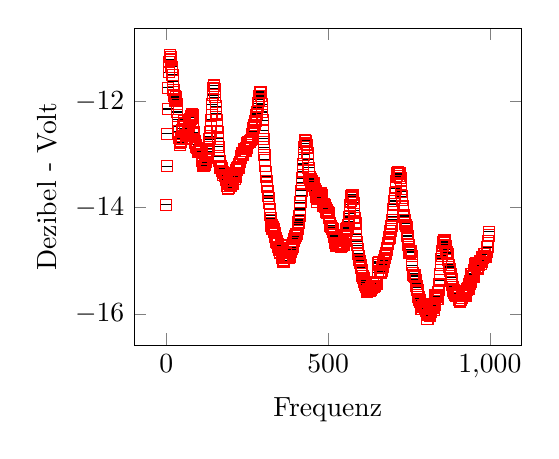
\begin{tikzpicture}
		\pgfplotsset{width=6.5cm,compat=1.3,legend style={font=\footnotesize}}
		\begin{axis}[xlabel={Frequenz},ylabel={Dezibel - Volt},legend cell align=left,legend pos=north west]
		\addplot+[only marks,color=red,mark=square,error bars/.cd,x dir=both,x explicit,y dir=both,y explicit,error bar style={color=black}] table[x=X,y=Y,x error=xerror,y error=yerror,row sep=\\]{			X	Y	xerror	yerror	\\			0.0	-13.944471	0	0	\\			1.464844	-13.218628	0	0	\\			2.929687	-12.60769	0	0	\\			4.394531	-12.141175	0	0	\\			5.859375	-11.741029	0	0	\\			7.324219	-11.452051	0	0	\\			8.789062	-11.249477	0	0	\\			10.253906	-11.158565	0	0	\\			11.71875	-11.117902	0	0	\\			13.183594	-11.161134	0	0	\\			14.648437	-11.211065	0	0	\\			16.113281	-11.346855	0	0	\\			17.578125	-11.398137	0	0	\\			19.042969	-11.4989	0	0	\\			20.507812	-11.616372	0	0	\\			21.972656	-11.784753	0	0	\\			23.4375	-11.873724	0	0	\\			24.902344	-11.901582	0	0	\\			26.367187	-11.996939	0	0	\\			27.832031	-11.952896	0	0	\\			29.296875	-11.923208	0	0	\\			30.761719	-11.966716	0	0	\\			32.226562	-12.051753	0	0	\\			33.691406	-12.198508	0	0	\\			35.15625	-12.344775	0	0	\\			36.621094	-12.473229	0	0	\\			38.085937	-12.559498	0	0	\\			39.550781	-12.692169	0	0	\\			41.015625	-12.779751	0	0	\\			42.480469	-12.817506	0	0	\\			43.945312	-12.759275	0	0	\\			45.410156	-12.750344	0	0	\\			46.875	-12.696855	0	0	\\			48.339844	-12.645603	0	0	\\			49.804687	-12.538719	0	0	\\			51.269531	-12.515609	0	0	\\			52.734375	-12.454646	0	0	\\			54.199219	-12.359051	0	0	\\			55.664062	-12.346734	0	0	\\			57.128906	-12.415251	0	0	\\			58.59375	-12.530745	0	0	\\			60.058594	-12.635092	0	0	\\			61.523437	-12.678688	0	0	\\			62.988281	-12.704896	0	0	\\			64.453125	-12.641397	0	0	\\			65.917969	-12.587232	0	0	\\			67.382812	-12.53973	0	0	\\			68.847656	-12.468172	0	0	\\			70.3125	-12.390512	0	0	\\			71.777344	-12.365978	0	0	\\			73.242187	-12.353352	0	0	\\			74.707031	-12.334407	0	0	\\			76.171875	-12.301089	0	0	\\			77.636719	-12.273698	0	0	\\			79.101562	-12.240015	0	0	\\			80.566406	-12.253447	0	0	\\			82.03125	-12.375394	0	0	\\			83.496094	-12.508262	0	0	\\			84.960937	-12.583697	0	0	\\			86.425781	-12.619764	0	0	\\			87.890625	-12.745579	0	0	\\			89.355469	-12.773291	0	0	\\			90.820312	-12.811458	0	0	\\			92.285156	-12.8547	0	0	\\			93.75	-12.880704	0	0	\\			95.214844	-12.881597	0	0	\\			96.679687	-12.943458	0	0	\\			98.144531	-12.954904	0	0	\\			99.609375	-12.944888	0	0	\\			101.074219	-12.930625	0	0	\\			102.539062	-12.944276	0	0	\\			104.003906	-12.913877	0	0	\\			105.46875	-12.896136	0	0	\\			106.933594	-12.904053	0	0	\\			108.398437	-12.941211	0	0	\\			109.863281	-13.017003	0	0	\\			111.328125	-13.118068	0	0	\\			112.792969	-13.181165	0	0	\\			114.257812	-13.210408	0	0	\\			115.722656	-13.222059	0	0	\\			117.1875	-13.206618	0	0	\\			118.652344	-13.18745	0	0	\\			120.117187	-13.160107	0	0	\\			121.582031	-13.141237	0	0	\\			123.046875	-13.085509	0	0	\\			124.511719	-13.056335	0	0	\\			125.976562	-13.000671	0	0	\\			127.441406	-12.942684	0	0	\\			128.90625	-12.951481	0	0	\\			130.371094	-12.894858	0	0	\\			131.835937	-12.798687	0	0	\\			133.300781	-12.709976	0	0	\\			134.765625	-12.652854	0	0	\\			136.230469	-12.579898	0	0	\\			137.695312	-12.478897	0	0	\\			139.160156	-12.349247	0	0	\\			140.625	-12.251687	0	0	\\			142.089844	-12.050942	0	0	\\			143.554687	-11.878436	0	0	\\			145.019531	-11.749454	0	0	\\			146.484375	-11.701087	0	0	\\			147.949219	-11.700373	0	0	\\			149.414062	-11.762814	0	0	\\			150.878906	-11.920982	0	0	\\			152.34375	-12.086076	0	0	\\			153.808594	-12.224746	0	0	\\			155.273437	-12.354517	0	0	\\			156.738281	-12.462491	0	0	\\			158.203125	-12.569243	0	0	\\			159.667969	-12.697632	0	0	\\			161.132812	-12.85369	0	0	\\			162.597656	-13.025272	0	0	\\			164.0625	-13.122604	0	0	\\			165.527344	-13.224956	0	0	\\			166.992187	-13.253829	0	0	\\			168.457031	-13.25797	0	0	\\			169.921875	-13.207248	0	0	\\			171.386719	-13.248703	0	0	\\			172.851562	-13.312195	0	0	\\			174.316406	-13.377979	0	0	\\			175.78125	-13.336645	0	0	\\			177.246094	-13.35217	0	0	\\			178.710937	-13.34573	0	0	\\			180.175781	-13.384513	0	0	\\			181.640625	-13.408233	0	0	\\			183.105469	-13.435046	0	0	\\			184.570312	-13.427732	0	0	\\			186.035156	-13.472448	0	0	\\			187.5	-13.545692	0	0	\\			188.964844	-13.596029	0	0	\\			190.429687	-13.639801	0	0	\\			191.894531	-13.628171	0	0	\\			193.359375	-13.557249	0	0	\\			194.824219	-13.501319	0	0	\\			196.289062	-13.529682	0	0	\\			197.753906	-13.59435	0	0	\\			199.21875	-13.596339	0	0	\\			200.683594	-13.563706	0	0	\\			202.148437	-13.538814	0	0	\\			203.613281	-13.536267	0	0	\\			205.078125	-13.544189	0	0	\\			206.542969	-13.494117	0	0	\\			208.007812	-13.405475	0	0	\\			209.472656	-13.363182	0	0	\\			210.9375	-13.385856	0	0	\\			212.402344	-13.46236	0	0	\\			213.867187	-13.416484	0	0	\\			215.332031	-13.368327	0	0	\\			216.796875	-13.296043	0	0	\\			218.261719	-13.263946	0	0	\\			219.726562	-13.257138	0	0	\\			221.191406	-13.240819	0	0	\\			222.65625	-13.249893	0	0	\\			224.121094	-13.256779	0	0	\\			225.585937	-13.180697	0	0	\\			227.050781	-13.137939	0	0	\\			228.515625	-13.13289	0	0	\\			229.980469	-13.068613	0	0	\\			231.445312	-13.03647	0	0	\\			232.910156	-12.97851	0	0	\\			234.375	-12.987958	0	0	\\			235.839844	-12.995954	0	0	\\			237.304687	-13.003028	0	0	\\			238.769531	-12.932255	0	0	\\			240.234375	-12.90124	0	0	\\			241.699219	-12.925771	0	0	\\			243.164062	-12.895974	0	0	\\			244.628906	-12.937637	0	0	\\			246.09375	-12.899736	0	0	\\			247.558594	-12.870586	0	0	\\			249.023437	-12.858518	0	0	\\			250.488281	-12.787242	0	0	\\			251.953125	-12.774146	0	0	\\			253.417969	-12.766766	0	0	\\			254.882812	-12.766072	0	0	\\			256.347656	-12.766291	0	0	\\			257.8125	-12.766131	0	0	\\			259.277344	-12.745827	0	0	\\			260.742187	-12.723559	0	0	\\			262.207031	-12.718322	0	0	\\			263.671875	-12.68439	0	0	\\			265.136719	-12.616666	0	0	\\			266.601562	-12.561203	0	0	\\			268.066406	-12.539476	0	0	\\			269.53125	-12.499734	0	0	\\			270.996094	-12.488675	0	0	\\			272.460937	-12.441403	0	0	\\			273.925781	-12.384141	0	0	\\			275.390625	-12.372125	0	0	\\			276.855469	-12.286503	0	0	\\			278.320312	-12.24962	0	0	\\			279.785156	-12.230826	0	0	\\			281.25	-12.202706	0	0	\\			282.714844	-12.102675	0	0	\\			284.179687	-12.037275	0	0	\\			285.644531	-11.963993	0	0	\\			287.109375	-11.890521	0	0	\\			288.574219	-11.844678	0	0	\\			290.039062	-11.814098	0	0	\\			291.503906	-11.823036	0	0	\\			292.96875	-11.902914	0	0	\\			294.433594	-12.050198	0	0	\\			295.898437	-12.197382	0	0	\\			297.363281	-12.356081	0	0	\\			298.828125	-12.546665	0	0	\\			300.292969	-12.701117	0	0	\\			301.757812	-12.860263	0	0	\\			303.222656	-13.000226	0	0	\\			304.6875	-13.100011	0	0	\\			306.152344	-13.218447	0	0	\\			307.617187	-13.323501	0	0	\\			309.082031	-13.422369	0	0	\\			310.546875	-13.501773	0	0	\\			312.011719	-13.600167	0	0	\\			313.476562	-13.68956	0	0	\\			314.941406	-13.776085	0	0	\\			316.40625	-13.825046	0	0	\\			317.871094	-13.914549	0	0	\\			319.335937	-14.017291	0	0	\\			320.800781	-14.143981	0	0	\\			322.265625	-14.201067	0	0	\\			323.730469	-14.283797	0	0	\\			325.195312	-14.333463	0	0	\\			326.660156	-14.362655	0	0	\\			328.125	-14.39513	0	0	\\			329.589844	-14.37248	0	0	\\			331.054687	-14.393551	0	0	\\			332.519531	-14.438617	0	0	\\			333.984375	-14.46365	0	0	\\			335.449219	-14.480571	0	0	\\			336.914062	-14.55467	0	0	\\			338.378906	-14.57541	0	0	\\			339.84375	-14.637146	0	0	\\			341.308594	-14.637175	0	0	\\			342.773437	-14.66142	0	0	\\			344.238281	-14.683445	0	0	\\			345.703125	-14.739505	0	0	\\			347.167969	-14.762295	0	0	\\			348.632812	-14.795823	0	0	\\			350.097656	-14.849707	0	0	\\			351.5625	-14.841125	0	0	\\			353.027344	-14.767082	0	0	\\			354.492187	-14.717885	0	0	\\			355.957031	-14.706983	0	0	\\			357.421875	-14.753139	0	0	\\			358.886719	-14.93686	0	0	\\			360.351562	-14.987807	0	0	\\			361.816406	-15.028744	0	0	\\			363.28125	-15.00958	0	0	\\			364.746094	-14.986256	0	0	\\			366.210937	-14.938313	0	0	\\			367.675781	-14.900853	0	0	\\			369.140625	-14.859244	0	0	\\			370.605469	-14.915338	0	0	\\			372.070312	-14.93831	0	0	\\			373.535156	-14.951109	0	0	\\			375.0	-14.919264	0	0	\\			376.464844	-14.925843	0	0	\\			377.929687	-14.927466	0	0	\\			379.394531	-14.944752	0	0	\\			380.859375	-14.917676	0	0	\\			382.324219	-14.911064	0	0	\\			383.789062	-14.833353	0	0	\\			385.253906	-14.794458	0	0	\\			386.71875	-14.777003	0	0	\\			388.183594	-14.762655	0	0	\\			389.648437	-14.741056	0	0	\\			391.113281	-14.722468	0	0	\\			392.578125	-14.656089	0	0	\\			394.042969	-14.624511	0	0	\\			395.507812	-14.584727	0	0	\\			396.972656	-14.573375	0	0	\\			398.4375	-14.538434	0	0	\\			399.902344	-14.52219	0	0	\\			401.367187	-14.490736	0	0	\\			402.832031	-14.497974	0	0	\\			404.296875	-14.497345	0	0	\\			405.761719	-14.403138	0	0	\\			407.226562	-14.314085	0	0	\\			408.691406	-14.276795	0	0	\\			410.15625	-14.230695	0	0	\\			411.621094	-14.149248	0	0	\\			413.085937	-14.022943	0	0	\\			414.550781	-13.896144	0	0	\\			416.015625	-13.765987	0	0	\\			417.480469	-13.683342	0	0	\\			418.945312	-13.53428	0	0	\\			420.410156	-13.444636	0	0	\\			421.875	-13.316637	0	0	\\			423.339844	-13.175632	0	0	\\			424.804687	-13.003827	0	0	\\			426.269531	-12.861132	0	0	\\			427.734375	-12.736735	0	0	\\			429.199219	-12.727476	0	0	\\			430.664062	-12.747351	0	0	\\			432.128906	-12.791325	0	0	\\			433.59375	-12.820658	0	0	\\			435.058594	-12.854948	0	0	\\			436.523437	-12.96389	0	0	\\			437.988281	-13.084389	0	0	\\			439.453125	-13.248909	0	0	\\			440.917969	-13.315121	0	0	\\			442.382812	-13.426718	0	0	\\			443.847656	-13.471992	0	0	\\			445.3125	-13.457287	0	0	\\			446.777344	-13.476225	0	0	\\			448.242187	-13.509281	0	0	\\			449.707031	-13.501175	0	0	\\			451.171875	-13.537795	0	0	\\			452.636719	-13.537614	0	0	\\			454.101562	-13.537497	0	0	\\			455.566406	-13.529049	0	0	\\			457.03125	-13.591064	0	0	\\			458.496094	-13.648225	0	0	\\			459.960937	-13.665812	0	0	\\			461.425781	-13.687221	0	0	\\			462.890625	-13.761158	0	0	\\			464.355469	-13.802799	0	0	\\			465.820312	-13.893707	0	0	\\			467.285156	-13.842652	0	0	\\			468.75	-13.814306	0	0	\\			470.214844	-13.778938	0	0	\\			471.679687	-13.781903	0	0	\\			473.144531	-13.802782	0	0	\\			474.609375	-13.782766	0	0	\\			476.074219	-13.750391	0	0	\\			477.539062	-13.729134	0	0	\\			479.003906	-13.769806	0	0	\\			480.46875	-13.767564	0	0	\\			481.933594	-13.822662	0	0	\\			483.398437	-13.941027	0	0	\\			484.863281	-13.967739	0	0	\\			486.328125	-13.95642	0	0	\\			487.792969	-13.93721	0	0	\\			489.257812	-13.944364	0	0	\\			490.722656	-13.992701	0	0	\\			492.1875	-14.011239	0	0	\\			493.652344	-14.074031	0	0	\\			495.117187	-14.058389	0	0	\\			496.582031	-14.05231	0	0	\\			498.046875	-14.102584	0	0	\\			499.511719	-14.08063	0	0	\\			500.976562	-14.095954	0	0	\\			502.441406	-14.141648	0	0	\\			503.90625	-14.199574	0	0	\\			505.371094	-14.292513	0	0	\\			506.835937	-14.342627	0	0	\\			508.300781	-14.346556	0	0	\\			509.765625	-14.3543	0	0	\\			511.230469	-14.378662	0	0	\\			512.695312	-14.39205	0	0	\\			514.160156	-14.401136	0	0	\\			515.625	-14.458383	0	0	\\			517.089844	-14.5145	0	0	\\			518.554687	-14.545935	0	0	\\			520.019531	-14.59685	0	0	\\			521.484375	-14.611129	0	0	\\			522.949219	-14.666533	0	0	\\			524.414062	-14.71703	0	0	\\			525.878906	-14.702909	0	0	\\			527.34375	-14.70853	0	0	\\			528.808594	-14.670805	0	0	\\			530.273437	-14.672267	0	0	\\			531.738281	-14.69602	0	0	\\			533.203125	-14.679773	0	0	\\			534.667969	-14.687149	0	0	\\			536.132812	-14.688838	0	0	\\			537.597656	-14.684397	0	0	\\			539.0625	-14.699907	0	0	\\			540.527344	-14.735897	0	0	\\			541.992187	-14.716112	0	0	\\			543.457031	-14.710752	0	0	\\			544.921875	-14.687977	0	0	\\			546.386719	-14.670953	0	0	\\			547.851562	-14.704329	0	0	\\			549.316406	-14.684968	0	0	\\			550.78125	-14.630869	0	0	\\			552.246094	-14.597656	0	0	\\			553.710937	-14.505954	0	0	\\			555.175781	-14.444022	0	0	\\			556.640625	-14.402177	0	0	\\			558.105469	-14.385234	0	0	\\			559.570312	-14.420059	0	0	\\			561.035156	-14.379676	0	0	\\			562.5	-14.333834	0	0	\\			563.964844	-14.255669	0	0	\\			565.429687	-14.173801	0	0	\\			566.894531	-14.102304	0	0	\\			568.359375	-13.943775	0	0	\\			569.824219	-13.865548	0	0	\\			571.289062	-13.788322	0	0	\\			572.753906	-13.758116	0	0	\\			574.21875	-13.754412	0	0	\\			575.683594	-13.767614	0	0	\\			577.148437	-13.810125	0	0	\\			578.613281	-13.907848	0	0	\\			580.078125	-14.04967	0	0	\\			581.542969	-14.199365	0	0	\\			583.007812	-14.271518	0	0	\\			584.472656	-14.296674	0	0	\\			585.9375	-14.386687	0	0	\\			587.402344	-14.510152	0	0	\\			588.867187	-14.640319	0	0	\\			590.332031	-14.70888	0	0	\\			591.796875	-14.774532	0	0	\\			593.261719	-14.861688	0	0	\\			594.726562	-14.910425	0	0	\\			596.191406	-14.98195	0	0	\\			597.65625	-14.996569	0	0	\\			599.121094	-15.037669	0	0	\\			600.585937	-15.077797	0	0	\\			602.050781	-15.131254	0	0	\\			603.515625	-15.176684	0	0	\\			604.980469	-15.217383	0	0	\\			606.445312	-15.289591	0	0	\\			607.910156	-15.323754	0	0	\\			609.375	-15.32428	0	0	\\			610.839844	-15.360672	0	0	\\			612.304687	-15.403515	0	0	\\			613.769531	-15.450175	0	0	\\			615.234375	-15.423166	0	0	\\			616.699219	-15.433057	0	0	\\			618.164062	-15.486894	0	0	\\			619.628906	-15.570838	0	0	\\			621.09375	-15.584244	0	0	\\			622.558594	-15.563721	0	0	\\			624.023437	-15.531904	0	0	\\			625.488281	-15.528757	0	0	\\			626.953125	-15.550579	0	0	\\			628.417969	-15.557608	0	0	\\			629.882812	-15.561039	0	0	\\			631.347656	-15.548705	0	0	\\			632.8125	-15.519282	0	0	\\			634.277344	-15.501333	0	0	\\			635.742187	-15.473194	0	0	\\			637.207031	-15.469528	0	0	\\			638.671875	-15.443163	0	0	\\			640.136719	-15.471451	0	0	\\			641.601562	-15.486887	0	0	\\			643.066406	-15.481984	0	0	\\			644.53125	-15.46822	0	0	\\			645.996094	-15.432798	0	0	\\			647.460937	-15.421824	0	0	\\			648.925781	-15.403651	0	0	\\			650.390625	-15.428911	0	0	\\			651.855469	-15.392459	0	0	\\			653.320312	-15.214365	0	0	\\			654.785156	-15.040799	0	0	\\			656.25	-15.019704	0	0	\\			657.714844	-15.082795	0	0	\\			659.179687	-15.193071	0	0	\\			660.644531	-15.217559	0	0	\\			662.109375	-15.23239	0	0	\\			663.574219	-15.23089	0	0	\\			665.039062	-15.184462	0	0	\\			666.503906	-15.132194	0	0	\\			667.96875	-15.107932	0	0	\\			669.433594	-15.070447	0	0	\\			670.898437	-15.050131	0	0	\\			672.363281	-15.010623	0	0	\\			673.828125	-14.989426	0	0	\\			675.292969	-14.946257	0	0	\\			676.757812	-14.907106	0	0	\\			678.222656	-14.874861	0	0	\\			679.6875	-14.850349	0	0	\\			681.152344	-14.798424	0	0	\\			682.617187	-14.763837	0	0	\\			684.082031	-14.682101	0	0	\\			685.546875	-14.656988	0	0	\\			687.011719	-14.59062	0	0	\\			688.476562	-14.546267	0	0	\\			689.941406	-14.566493	0	0	\\			691.40625	-14.501333	0	0	\\			692.871094	-14.441339	0	0	\\			694.335937	-14.403616	0	0	\\			695.800781	-14.33902	0	0	\\			697.265625	-14.295951	0	0	\\			698.730469	-14.223634	0	0	\\			700.195312	-14.158067	0	0	\\			701.660156	-14.027315	0	0	\\			703.125	-13.932481	0	0	\\			704.589844	-13.872199	0	0	\\			706.054687	-13.822815	0	0	\\			707.519531	-13.718135	0	0	\\			708.984375	-13.63279	0	0	\\			710.449219	-13.501634	0	0	\\			711.914062	-13.402344	0	0	\\			713.378906	-13.348868	0	0	\\			714.84375	-13.37144	0	0	\\			716.308594	-13.336207	0	0	\\			717.773437	-13.405103	0	0	\\			719.238281	-13.344171	0	0	\\			720.703125	-13.342639	0	0	\\			722.167969	-13.403023	0	0	\\			723.632812	-13.444673	0	0	\\			725.097656	-13.547066	0	0	\\			726.5625	-13.695242	0	0	\\			728.027344	-13.786537	0	0	\\			729.492187	-13.857549	0	0	\\			730.957031	-13.963897	0	0	\\			732.421875	-14.03139	0	0	\\			733.886719	-14.140159	0	0	\\			735.351562	-14.16651	0	0	\\			736.816406	-14.230729	0	0	\\			738.28125	-14.296164	0	0	\\			739.746094	-14.334641	0	0	\\			741.210937	-14.329275	0	0	\\			742.675781	-14.370539	0	0	\\			744.140625	-14.467219	0	0	\\			745.605469	-14.531827	0	0	\\			747.070312	-14.583495	0	0	\\			748.535156	-14.697794	0	0	\\			750.0	-14.786569	0	0	\\			751.464844	-14.849499	0	0	\\			752.929687	-14.848566	0	0	\\			754.394531	-14.816746	0	0	\\			755.859375	-14.807675	0	0	\\			757.324219	-14.823869	0	0	\\			758.789062	-14.908406	0	0	\\			760.253906	-15.085575	0	0	\\			761.71875	-15.234924	0	0	\\			763.183594	-15.261746	0	0	\\			764.648437	-15.292001	0	0	\\			766.113281	-15.273074	0	0	\\			767.578125	-15.268497	0	0	\\			769.042969	-15.294751	0	0	\\			770.507812	-15.352574	0	0	\\			771.972656	-15.427966	0	0	\\			773.4375	-15.478346	0	0	\\			774.902344	-15.509839	0	0	\\			776.367187	-15.54485	0	0	\\			777.832031	-15.583446	0	0	\\			779.296875	-15.687774	0	0	\\			780.761719	-15.717089	0	0	\\			782.226562	-15.736434	0	0	\\			783.691406	-15.764384	0	0	\\			785.15625	-15.776802	0	0	\\			786.621094	-15.837355	0	0	\\			788.085937	-15.905927	0	0	\\			789.550781	-15.9109	0	0	\\			791.015625	-15.875569	0	0	\\			792.480469	-15.848251	0	0	\\			793.945312	-15.847396	0	0	\\			795.410156	-15.823541	0	0	\\			796.875	-15.829923	0	0	\\			798.339844	-15.82127	0	0	\\			799.804687	-15.847274	0	0	\\			801.269531	-15.876796	0	0	\\			802.734375	-15.905272	0	0	\\			804.199219	-15.94542	0	0	\\			805.664062	-16.023803	0	0	\\			807.128906	-16.089433	0	0	\\			808.59375	-16.016709	0	0	\\			810.058594	-16.013508	0	0	\\			811.523437	-15.990251	0	0	\\			812.988281	-16.007226	0	0	\\			814.453125	-15.986158	0	0	\\			815.917969	-16.034829	0	0	\\			817.382812	-15.968	0	0	\\			818.847656	-15.892651	0	0	\\			820.3125	-15.870638	0	0	\\			821.777344	-15.848883	0	0	\\			823.242187	-15.852079	0	0	\\			824.707031	-15.883786	0	0	\\			826.171875	-15.918997	0	0	\\			827.636719	-15.923488	0	0	\\			829.101562	-15.821191	0	0	\\			830.566406	-15.70647	0	0	\\			832.03125	-15.652331	0	0	\\			833.496094	-15.661485	0	0	\\			834.960937	-15.665487	0	0	\\			836.425781	-15.682887	0	0	\\			837.890625	-15.709029	0	0	\\			839.355469	-15.660995	0	0	\\			840.820312	-15.585292	0	0	\\			842.285156	-15.553211	0	0	\\			843.75	-15.437059	0	0	\\			845.214844	-15.36853	0	0	\\			846.679687	-15.25177	0	0	\\			848.144531	-15.072892	0	0	\\			849.609375	-14.96344	0	0	\\			851.074219	-14.906902	0	0	\\			852.539062	-14.822843	0	0	\\			854.003906	-14.720787	0	0	\\			855.46875	-14.694269	0	0	\\			856.933594	-14.654292	0	0	\\			858.398437	-14.629808	0	0	\\			859.863281	-14.616036	0	0	\\			861.328125	-14.632258	0	0	\\			862.792969	-14.720911	0	0	\\			864.257812	-14.779922	0	0	\\			865.722656	-14.835606	0	0	\\			867.1875	-14.857485	0	0	\\			868.652344	-14.842156	0	0	\\			870.117187	-14.872574	0	0	\\			871.582031	-14.976067	0	0	\\			873.046875	-15.078117	0	0	\\			874.511719	-15.116492	0	0	\\			875.976562	-15.145783	0	0	\\			877.441406	-15.183484	0	0	\\			878.90625	-15.249494	0	0	\\			880.371094	-15.315832	0	0	\\			881.835937	-15.352098	0	0	\\			883.300781	-15.45737	0	0	\\			884.765625	-15.489204	0	0	\\			886.230469	-15.499059	0	0	\\			887.695312	-15.558827	0	0	\\			889.160156	-15.604945	0	0	\\			890.625	-15.600385	0	0	\\			892.089844	-15.630406	0	0	\\			893.554687	-15.64477	0	0	\\			895.019531	-15.657829	0	0	\\			896.484375	-15.661049	0	0	\\			897.949219	-15.638733	0	0	\\			899.414062	-15.642555	0	0	\\			900.878906	-15.634869	0	0	\\			902.34375	-15.593759	0	0	\\			903.808594	-15.625502	0	0	\\			905.273437	-15.741353	0	0	\\			906.738281	-15.768944	0	0	\\			908.203125	-15.763954	0	0	\\			909.667969	-15.741365	0	0	\\			911.132812	-15.740473	0	0	\\			912.597656	-15.694883	0	0	\\			914.0625	-15.641633	0	0	\\			915.527344	-15.632309	0	0	\\			916.992187	-15.619794	0	0	\\			918.457031	-15.627323	0	0	\\			919.921875	-15.613578	0	0	\\			921.386719	-15.616595	0	0	\\			922.851562	-15.601726	0	0	\\			924.316406	-15.641107	0	0	\\			925.78125	-15.654087	0	0	\\			927.246094	-15.563979	0	0	\\			928.710937	-15.540728	0	0	\\			930.175781	-15.522229	0	0	\\			931.640625	-15.504444	0	0	\\			933.105469	-15.528893	0	0	\\			934.570312	-15.523504	0	0	\\			936.035156	-15.435019	0	0	\\			937.5	-15.425332	0	0	\\			938.964844	-15.382462	0	0	\\			940.429687	-15.38911	0	0	\\			941.894531	-15.312656	0	0	\\			943.359375	-15.244778	0	0	\\			944.824219	-15.255819	0	0	\\			946.289062	-15.287437	0	0	\\			947.753906	-15.289783	0	0	\\			949.21875	-15.309993	0	0	\\			950.683594	-15.273668	0	0	\\			952.148437	-15.170406	0	0	\\			953.613281	-15.090493	0	0	\\			955.078125	-15.056735	0	0	\\			956.542969	-15.045634	0	0	\\			958.007812	-15.072196	0	0	\\			959.472656	-15.111009	0	0	\\			960.9375	-15.138774	0	0	\\			962.402344	-15.143305	0	0	\\			963.867187	-15.115052	0	0	\\			965.332031	-15.069476	0	0	\\			966.796875	-15.036253	0	0	\\			968.261719	-15.000561	0	0	\\			969.726562	-15.012249	0	0	\\			971.191406	-15.06547	0	0	\\			972.65625	-15.06399	0	0	\\			974.121094	-15.022663	0	0	\\			975.585937	-14.959842	0	0	\\			977.050781	-14.925161	0	0	\\			978.515625	-14.936986	0	0	\\			979.980469	-14.94617	0	0	\\			981.445312	-14.931677	0	0	\\			982.910156	-14.877084	0	0	\\			984.375	-14.869712	0	0	\\			985.839844	-14.913588	0	0	\\			987.304687	-14.934401	0	0	\\			988.769531	-14.930792	0	0	\\			990.234375	-14.833539	0	0	\\			991.699219	-14.747825	0	0	\\			993.164062	-14.730986	0	0	\\			994.628906	-14.624443	0	0	\\			996.09375	-14.521525	0	0	\\			997.558594	-14.450173	0	0	\\		};		% \addlegendentry{Messpunkte Datensatz 0}
		\end{axis}
		\end{tikzpicture}	\caption{Umgebung}
	\label{fig:Umgebungsmessung}\end{figure}

        \subsubsection*{68 degrees}
            \begin{table}[H]
	\centering
	\begin{tabular}{cccccc}
		n & $\nu$ & c & C(c) & $\kappa$ & f\\
		\hline
		0.0 & 11.2(50) & 22.4(224) & 22.3(223) & 0.01(00) & -2.02(-02)	\\
		1.0 & 146.8(50) & 146.8(1468) & 146.62(1466) & 0.38(004) & -3.23(-032)	\\
		2.0 & 288.8(50) & 192.53(1925) & 192.37(1924) & 0.65(007) & -5.78(-058)	\\
		3.0 & 428.8(50) & 214.4(2144) & 214.25(2142) & 0.81(008) & -10.58(-106)	\\
		4.0 & 542.8(50) & 217.12(2171) & 216.98(217) & 0.83(008) & -11.89(-119)	\\
		5.0 & 712.8(50) & 237.6(2376) & 237.47(2375) & 1.0(01) & -508.64(-5086)	\\
		6.0 & 856.0(50) & 244.57(2446) & 244.45(2444) & 1.06(011) & 36.12(361)	\\
		7.0 & 997.0(50) & 249.25(2493) & 249.14(2491) & 1.1(011) & 20.8(208)	\\
		0.0(00) & 498.02(177) & 190.58(719) & 190.45(718) & 0.73(003) & -60.65(638)	\\
	\end{tabular}
\end{table}
            \begin{table}[H]
	\centering
	\begin{tabular}{cccccc}
		n & $\nu$ & c & C(c) & $\kappa$ & f\\
		\hline
		0.0 & 11.2(50) & 22.4(224) & 22.3(223) & 0.01(00) & -2.02(-02)	\\
		1.0 & 146.8(50) & 146.8(1468) & 146.62(1466) & 0.38(004) & -3.23(-032)	\\
		2.0 & 288.8(50) & 192.53(1925) & 192.37(1924) & 0.65(007) & -5.78(-058)	\\
		3.0 & 428.8(50) & 214.4(2144) & 214.25(2142) & 0.81(008) & -10.58(-106)	\\
		4.0 & 542.8(50) & 217.12(2171) & 216.98(217) & 0.83(008) & -11.89(-119)	\\
		5.0 & 712.8(50) & 237.6(2376) & 237.47(2375) & 1.0(01) & -508.64(-5086)	\\
		6.0 & 856.0(50) & 244.57(2446) & 244.45(2444) & 1.06(011) & 36.12(361)	\\
		7.0 & 997.0(50) & 249.25(2493) & 249.14(2491) & 1.1(011) & 20.8(208)	\\
		0.0(00) & 498.02(177) & 190.58(719) & 190.45(718) & 0.73(003) & -60.65(638)	\\
	\end{tabular}
\end{table}

        \subsubsection*{63 degrees}
            \begin{table}[H]
	\centering
	\begin{tabular}{cccccc}
		$\nu$ & c & C(c) & $\kappa$ & f\\
		\hline
		0.0 & 11.0(50) & 22.0(22) & 21.9(219) & 0.01(00) & -2.02(-02)	\\
		1.0 & 145.0(50) & 145.0(145) & 144.82(1448) & 0.37(004) & -3.18(-032)	\\
		2.0 & 287.0(50) & 191.33(1913) & 191.17(1912) & 0.65(006) & -5.65(-056)	\\
		3.0 & 426.0(50) & 213.0(213) & 212.85(2128) & 0.8(008) & -10.02(-10)	\\
		4.0 & 566.0(50) & 226.4(2264) & 226.26(2263) & 0.9(009) & -20.92(-209)	\\
		5.0 & 768.0(50) & 256.0(256) & 255.87(2559) & 1.16(012) & 12.79(128)	\\
		6.0 & 854.0(50) & 244.0(244) & 243.88(2439) & 1.05(011) & 39.64(396)	\\
		7.0 & 987.0(50) & 246.75(2468) & 246.64(2466) & 1.07(011) & 26.93(269)	\\
		0.0(00) & 505.5(177) & 193.06(73) & 192.92(729) & 0.75(003) & 4.7(069)	\\
	\end{tabular}
\end{table}
            \begin{table}[H]
	\centering
	\begin{tabular}{cccccc}
		$\nu$ & c & C(c) & $\kappa$ & f\\
		\hline
		0.0 & 11.0(50) & 22.0(22) & 21.9(219) & 0.01(00) & -2.02(-02)	\\
		1.0 & 145.0(50) & 145.0(145) & 144.82(1448) & 0.37(004) & -3.18(-032)	\\
		2.0 & 287.0(50) & 191.33(1913) & 191.17(1912) & 0.65(006) & -5.65(-056)	\\
		3.0 & 426.0(50) & 213.0(213) & 212.85(2128) & 0.8(008) & -10.02(-10)	\\
		4.0 & 566.0(50) & 226.4(2264) & 226.26(2263) & 0.9(009) & -20.92(-209)	\\
		5.0 & 768.0(50) & 256.0(256) & 255.87(2559) & 1.16(012) & 12.79(128)	\\
		6.0 & 854.0(50) & 244.0(244) & 243.88(2439) & 1.05(011) & 39.64(396)	\\
		7.0 & 987.0(50) & 246.75(2468) & 246.64(2466) & 1.07(011) & 26.93(269)	\\
		0.0(00) & 505.5(177) & 193.06(73) & 192.92(729) & 0.75(003) & 4.7(069)	\\
	\end{tabular}
\end{table}
        
        \subsubsection*{58 degrees}
            \begin{table}[H]
	\centering
	\begin{tabular}{cccccc}
		n & $\nu$ & c & C(c) & $\kappa$ & f\\
		\hline
		0.0 & 12.0(50) & 24.0(24) & 23.9(239) & 0.01(00) & -2.02(-02)	\\
		1.0 & 143.0(50) & 143.0(143) & 142.83(1428) & 0.36(004) & -3.13(-031)	\\
		2.0 & 286.0(50) & 190.67(1907) & 190.5(1905) & 0.64(006) & -5.58(-056)	\\
		3.0 & 426.0(50) & 213.0(213) & 212.85(2128) & 0.8(008) & -10.02(-10)	\\
		4.0 & 563.0(50) & 225.2(2252) & 225.06(2251) & 0.89(009) & -19.01(-19)	\\
		5.0 & 703.0(50) & 234.33(2343) & 234.2(2342) & 0.97(01) & -64.24(-642)	\\
		6.0 & 844.0(50) & 241.14(2411) & 241.02(241) & 1.03(01) & 76.94(769)	\\
		7.0 & 980.0(50) & 245.0(245) & 244.89(2449) & 1.06(011) & 33.85(339)	\\
		0.0(00) & 494.62(177) & 189.54(714) & 189.41(714) & 0.72(003) & 0.85(135)	\\
	\end{tabular}
\end{table}
            \begin{table}[H]
	\centering
	\begin{tabular}{cccccc}
		n & $\nu$ & c & C(c) & $\kappa$ & f\\
		\hline
		0.0 & 12.0(50) & 24.0(24) & 23.9(239) & 0.01(00) & -2.02(-02)	\\
		1.0 & 143.0(50) & 143.0(143) & 142.83(1428) & 0.36(004) & -3.13(-031)	\\
		2.0 & 286.0(50) & 190.67(1907) & 190.5(1905) & 0.64(006) & -5.58(-056)	\\
		3.0 & 426.0(50) & 213.0(213) & 212.85(2128) & 0.8(008) & -10.02(-10)	\\
		4.0 & 563.0(50) & 225.2(2252) & 225.06(2251) & 0.89(009) & -19.01(-19)	\\
		5.0 & 703.0(50) & 234.33(2343) & 234.2(2342) & 0.97(01) & -64.24(-642)	\\
		6.0 & 844.0(50) & 241.14(2411) & 241.02(241) & 1.03(01) & 76.94(769)	\\
		7.0 & 980.0(50) & 245.0(245) & 244.89(2449) & 1.06(011) & 33.85(339)	\\
		0.0(00) & 494.62(177) & 189.54(714) & 189.41(714) & 0.72(003) & 0.85(135)	\\
	\end{tabular}
\end{table}
        
        \subsubsection*{53 degrees}
            \begin{table}[H]
	\centering
	\begin{tabular}{ccccc}
		c & C(c) & $\kappa$ & f\\
		\hline
		11 & 142 & 283 & 420 & 580 & 698 & 838 & 976	\\
		22.0 & 142.0 & 188.66666666666666 & 210.0 & 232.0 & 232.66666666666666 & 239.42857142857142 & 244.0	\\
		21.903421669199755 & 141.8265007790702 & 188.50337827345564 & 209.85080715134757 & 231.85974209588315 & 232.53844547364938 & 239.30814901653858 & 243.88628486420507	\\
		0.008539676865116362 & 0.35577281881860795 & 0.6280387331958714 & 0.7780986565116352 & 0.9496685280744278 & 0.9551342349385102 & 1.011458397784917 & 1.0504508302511726	\\
		-2.0172264621505276 & -3.1044949024540918 & -5.376903937294046 & -9.013014380892509 & -39.73656886008631 & -44.57741882388376 & 174.54447275627479 & 39.642558706028744	\\
	\end{tabular}
\end{table}
            \begin{table}[H]
	\centering
	\begin{tabular}{ccccc}
		c & C(c) & $\kappa$ & f\\
		\hline
		11 & 142 & 283 & 420 & 580 & 698 & 838 & 976	\\
		22.0 & 142.0 & 188.66666666666666 & 210.0 & 232.0 & 232.66666666666666 & 239.42857142857142 & 244.0	\\
		21.903421669199755 & 141.8265007790702 & 188.50337827345564 & 209.85080715134757 & 231.85974209588315 & 232.53844547364938 & 239.30814901653858 & 243.88628486420507	\\
		0.008539676865116362 & 0.35577281881860795 & 0.6280387331958714 & 0.7780986565116352 & 0.9496685280744278 & 0.9551342349385102 & 1.011458397784917 & 1.0504508302511726	\\
		-2.0172264621505276 & -3.1044949024540918 & -5.376903937294046 & -9.013014380892509 & -39.73656886008631 & -44.57741882388376 & 174.54447275627479 & 39.642558706028744	\\
	\end{tabular}
\end{table}
        
        \subsubsection*{38 degrees}
            \begin{table}[H]
	\centering
	\begin{tabular}{ccccc}
		c & C(c) & $\kappa$ & f\\
		\hline
		8.7 & 139 & 277 & 413 & 550 & 688 & 824 & 960	\\
		17.4 & 139.0 & 184.66666666666666 & 206.5 & 220.0 & 229.33333333333331 & 235.42857142857142 & 240.0	\\
		17.314109925630376 & 138.82834330089852 & 184.50511851915425 & 206.3520556490178 & 219.86341761475094 & 229.2060339437362 & 235.3091591684564 & 239.88722080716468	\\
		0.005341885470418656 & 0.340898960146515 & 0.6016904189012976 & 0.752378173143612 & 0.8539676865116361 & 0.927962535822231 & 0.977944955164319 & 1.0162921227907071	\\
		-2.0107411489282327 & -3.0344361168730525 & -5.02121991261966 & -8.076832423823163 & -13.695598954948856 & -27.763331522394235 & -90.68220059858454 & 122.75871141486735	\\
	\end{tabular}
\end{table}
            \begin{table}[H]
	\centering
	\begin{tabular}{ccccc}
		c & C(c) & $\kappa$ & f\\
		\hline
		8.7 & 139 & 277 & 413 & 550 & 688 & 824 & 960	\\
		17.4 & 139.0 & 184.66666666666666 & 206.5 & 220.0 & 229.33333333333331 & 235.42857142857142 & 240.0	\\
		17.314109925630376 & 138.82834330089852 & 184.50511851915425 & 206.3520556490178 & 219.86341761475094 & 229.2060339437362 & 235.3091591684564 & 239.88722080716468	\\
		0.005341885470418656 & 0.340898960146515 & 0.6016904189012976 & 0.752378173143612 & 0.8539676865116361 & 0.927962535822231 & 0.977944955164319 & 1.0162921227907071	\\
		-2.0107411489282327 & -3.0344361168730525 & -5.02121991261966 & -8.076832423823163 & -13.695598954948856 & -27.763331522394235 & -90.68220059858454 & 122.75871141486735	\\
	\end{tabular}
\end{table}
        
        \subsubsection*{31 degrees}
            \begin{figure}[H]
	\centering
	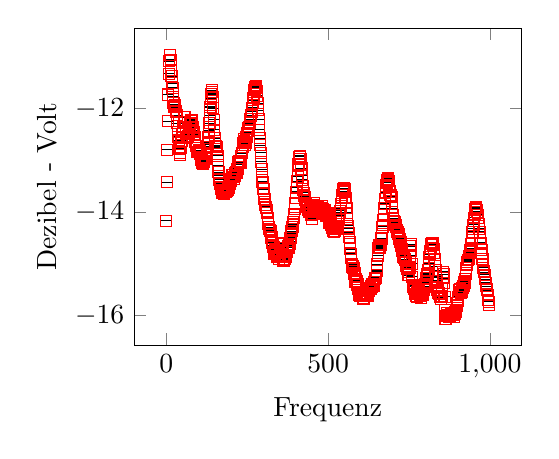
\begin{tikzpicture}
		\pgfplotsset{width=6.5cm,compat=1.3,legend style={font=\footnotesize}}
		\begin{axis}[xlabel={Frequenz},ylabel={Dezibel - Volt},legend cell align=left,legend pos=north west]
		\addplot+[only marks,color=red,mark=square,error bars/.cd,x dir=both,x explicit,y dir=both,y explicit,error bar style={color=black}] table[x=X,y=Y,x error=xerror,y error=yerror,row sep=\\]{			X	Y	xerror	yerror	\\			0.0	-14.164919	0	0	\\			1.464844	-13.423461	0	0	\\			2.929687	-12.795189	0	0	\\			4.394531	-12.245261	0	0	\\			5.859375	-11.730946	0	0	\\			7.324219	-11.329506	0	0	\\			8.789062	-11.085836	0	0	\\			10.253906	-10.961078	0	0	\\			11.71875	-10.973411	0	0	\\			13.183594	-11.064258	0	0	\\			14.648437	-11.258652	0	0	\\			16.113281	-11.375012	0	0	\\			17.578125	-11.516236	0	0	\\			19.042969	-11.597615	0	0	\\			20.507812	-11.773958	0	0	\\			21.972656	-11.89112	0	0	\\			23.4375	-11.958305	0	0	\\			24.902344	-11.977169	0	0	\\			26.367187	-11.933453	0	0	\\			27.832031	-11.946653	0	0	\\			29.296875	-12.067268	0	0	\\			30.761719	-12.043032	0	0	\\			32.226562	-12.130557	0	0	\\			33.691406	-12.287193	0	0	\\			35.15625	-12.452247	0	0	\\			36.621094	-12.543868	0	0	\\			38.085937	-12.618053	0	0	\\			39.550781	-12.772086	0	0	\\			41.015625	-12.893981	0	0	\\			42.480469	-12.850435	0	0	\\			43.945312	-12.752557	0	0	\\			45.410156	-12.653793	0	0	\\			46.875	-12.621641	0	0	\\			48.339844	-12.543832	0	0	\\			49.804687	-12.496791	0	0	\\			51.269531	-12.436894	0	0	\\			52.734375	-12.362595	0	0	\\			54.199219	-12.259872	0	0	\\			55.664062	-12.163448	0	0	\\			57.128906	-12.168667	0	0	\\			58.59375	-12.270183	0	0	\\			60.058594	-12.374486	0	0	\\			61.523437	-12.471527	0	0	\\			62.988281	-12.556238	0	0	\\			64.453125	-12.559223	0	0	\\			65.917969	-12.538605	0	0	\\			67.382812	-12.537811	0	0	\\			68.847656	-12.462484	0	0	\\			70.3125	-12.460954	0	0	\\			71.777344	-12.368802	0	0	\\			73.242187	-12.301627	0	0	\\			74.707031	-12.284165	0	0	\\			76.171875	-12.233723	0	0	\\			77.636719	-12.215283	0	0	\\			79.101562	-12.245056	0	0	\\			80.566406	-12.35783	0	0	\\			82.03125	-12.370201	0	0	\\			83.496094	-12.41712	0	0	\\			84.960937	-12.449146	0	0	\\			86.425781	-12.496071	0	0	\\			87.890625	-12.546374	0	0	\\			89.355469	-12.652713	0	0	\\			90.820312	-12.725718	0	0	\\			92.285156	-12.726218	0	0	\\			93.75	-12.755596	0	0	\\			95.214844	-12.835961	0	0	\\			96.679687	-12.832034	0	0	\\			98.144531	-12.833287	0	0	\\			99.609375	-12.847665	0	0	\\			101.074219	-12.808451	0	0	\\			102.539062	-12.823208	0	0	\\			104.003906	-12.833791	0	0	\\			105.46875	-12.871948	0	0	\\			106.933594	-12.967018	0	0	\\			108.398437	-12.999821	0	0	\\			109.863281	-13.033468	0	0	\\			111.328125	-13.055743	0	0	\\			112.792969	-13.065415	0	0	\\			114.257812	-13.051182	0	0	\\			115.722656	-13.015323	0	0	\\			117.1875	-13.033619	0	0	\\			118.652344	-12.974896	0	0	\\			120.117187	-12.933172	0	0	\\			121.582031	-12.963765	0	0	\\			123.046875	-12.965085	0	0	\\			124.511719	-12.859611	0	0	\\			125.976562	-12.738025	0	0	\\			127.441406	-12.690433	0	0	\\			128.90625	-12.661973	0	0	\\			130.371094	-12.560732	0	0	\\			131.835937	-12.429006	0	0	\\			133.300781	-12.285832	0	0	\\			134.765625	-12.138548	0	0	\\			136.230469	-11.972467	0	0	\\			137.695312	-11.806641	0	0	\\			139.160156	-11.721522	0	0	\\			140.625	-11.647183	0	0	\\			142.089844	-11.678916	0	0	\\			143.554687	-11.786087	0	0	\\			145.019531	-11.993779	0	0	\\			146.484375	-12.214814	0	0	\\			147.949219	-12.413501	0	0	\\			149.414062	-12.572942	0	0	\\			150.878906	-12.66897	0	0	\\			152.34375	-12.722298	0	0	\\			153.808594	-12.731719	0	0	\\			155.273437	-12.746778	0	0	\\			156.738281	-12.780426	0	0	\\			158.203125	-12.911675	0	0	\\			159.667969	-13.095085	0	0	\\			161.132812	-13.229077	0	0	\\			162.597656	-13.296058	0	0	\\			164.0625	-13.37067	0	0	\\			165.527344	-13.432754	0	0	\\			166.992187	-13.455957	0	0	\\			168.457031	-13.516274	0	0	\\			169.921875	-13.543134	0	0	\\			171.386719	-13.59857	0	0	\\			172.851562	-13.619785	0	0	\\			174.316406	-13.623	0	0	\\			175.78125	-13.632694	0	0	\\			177.246094	-13.644167	0	0	\\			178.710937	-13.613107	0	0	\\			180.175781	-13.6084	0	0	\\			181.640625	-13.610685	0	0	\\			183.105469	-13.615313	0	0	\\			184.570312	-13.600286	0	0	\\			186.035156	-13.577838	0	0	\\			187.5	-13.594874	0	0	\\			188.964844	-13.566325	0	0	\\			190.429687	-13.546297	0	0	\\			191.894531	-13.537756	0	0	\\			193.359375	-13.521826	0	0	\\			194.824219	-13.499905	0	0	\\			196.289062	-13.458123	0	0	\\			197.753906	-13.422541	0	0	\\			199.21875	-13.38834	0	0	\\			200.683594	-13.372364	0	0	\\			202.148437	-13.3292	0	0	\\			203.613281	-13.289784	0	0	\\			205.078125	-13.278719	0	0	\\			206.542969	-13.292925	0	0	\\			208.007812	-13.330059	0	0	\\			209.472656	-13.353241	0	0	\\			210.9375	-13.299781	0	0	\\			212.402344	-13.24685	0	0	\\			213.867187	-13.249435	0	0	\\			215.332031	-13.230795	0	0	\\			216.796875	-13.233479	0	0	\\			218.261719	-13.247204	0	0	\\			219.726562	-13.160436	0	0	\\			221.191406	-13.073816	0	0	\\			222.65625	-13.038491	0	0	\\			224.121094	-13.022263	0	0	\\			225.585937	-13.026715	0	0	\\			227.050781	-13.024103	0	0	\\			228.515625	-13.043439	0	0	\\			229.980469	-13.050436	0	0	\\			231.445312	-12.918389	0	0	\\			232.910156	-12.858723	0	0	\\			234.375	-12.861137	0	0	\\			235.839844	-12.740974	0	0	\\			237.304687	-12.67296	0	0	\\			238.769531	-12.621315	0	0	\\			240.234375	-12.595089	0	0	\\			241.699219	-12.646465	0	0	\\			243.164062	-12.703273	0	0	\\			244.628906	-12.673192	0	0	\\			246.09375	-12.601189	0	0	\\			247.558594	-12.551348	0	0	\\			249.023437	-12.503134	0	0	\\			250.488281	-12.468332	0	0	\\			251.953125	-12.43925	0	0	\\			253.417969	-12.385239	0	0	\\			254.882812	-12.368733	0	0	\\			256.347656	-12.377916	0	0	\\			257.8125	-12.284425	0	0	\\			259.277344	-12.210097	0	0	\\			260.742187	-12.144817	0	0	\\			262.207031	-12.127846	0	0	\\			263.671875	-12.057526	0	0	\\			265.136719	-11.99061	0	0	\\			266.601562	-11.897866	0	0	\\			268.066406	-11.838762	0	0	\\			269.53125	-11.791543	0	0	\\			270.996094	-11.728372	0	0	\\			272.460937	-11.649819	0	0	\\			273.925781	-11.615564	0	0	\\			275.390625	-11.594229	0	0	\\			276.855469	-11.56865	0	0	\\			278.320312	-11.610882	0	0	\\			279.785156	-11.657624	0	0	\\			281.25	-11.752055	0	0	\\			282.714844	-11.898074	0	0	\\			284.179687	-12.034184	0	0	\\			285.644531	-12.206844	0	0	\\			287.109375	-12.410667	0	0	\\			288.574219	-12.573703	0	0	\\			290.039062	-12.709421	0	0	\\			291.503906	-12.852396	0	0	\\			292.96875	-13.02938	0	0	\\			294.433594	-13.173633	0	0	\\			295.898437	-13.316868	0	0	\\			297.363281	-13.410936	0	0	\\			298.828125	-13.438397	0	0	\\			300.292969	-13.555132	0	0	\\			301.757812	-13.639437	0	0	\\			303.222656	-13.739624	0	0	\\			304.6875	-13.802883	0	0	\\			306.152344	-13.854175	0	0	\\			307.617187	-13.895003	0	0	\\			309.082031	-13.912361	0	0	\\			310.546875	-13.970285	0	0	\\			312.011719	-14.019984	0	0	\\			313.476562	-14.105786	0	0	\\			314.941406	-14.218993	0	0	\\			316.40625	-14.289461	0	0	\\			317.871094	-14.331567	0	0	\\			319.335937	-14.36875	0	0	\\			320.800781	-14.350113	0	0	\\			322.265625	-14.372686	0	0	\\			323.730469	-14.438382	0	0	\\			325.195312	-14.490969	0	0	\\			326.660156	-14.549839	0	0	\\			328.125	-14.594446	0	0	\\			329.589844	-14.640019	0	0	\\			331.054687	-14.676335	0	0	\\			332.519531	-14.778669	0	0	\\			333.984375	-14.805493	0	0	\\			335.449219	-14.79087	0	0	\\			336.914062	-14.725665	0	0	\\			338.378906	-14.751975	0	0	\\			339.84375	-14.795754	0	0	\\			341.308594	-14.850716	0	0	\\			342.773437	-14.865397	0	0	\\			344.238281	-14.8571	0	0	\\			345.703125	-14.87169	0	0	\\			347.167969	-14.89667	0	0	\\			348.632812	-14.91024	0	0	\\			350.097656	-14.866378	0	0	\\			351.5625	-14.822433	0	0	\\			353.027344	-14.697795	0	0	\\			354.492187	-14.606772	0	0	\\			355.957031	-14.603702	0	0	\\			357.421875	-14.684673	0	0	\\			358.886719	-14.743253	0	0	\\			360.351562	-14.822318	0	0	\\			361.816406	-14.944231	0	0	\\			363.28125	-14.943737	0	0	\\			364.746094	-14.917809	0	0	\\			366.210937	-14.901368	0	0	\\			367.675781	-14.908925	0	0	\\			369.140625	-14.873556	0	0	\\			370.605469	-14.848899	0	0	\\			372.070312	-14.768765	0	0	\\			373.535156	-14.726537	0	0	\\			375.0	-14.675093	0	0	\\			376.464844	-14.650801	0	0	\\			377.929687	-14.686325	0	0	\\			379.394531	-14.685237	0	0	\\			380.859375	-14.615952	0	0	\\			382.324219	-14.559062	0	0	\\			383.789062	-14.498126	0	0	\\			385.253906	-14.416506	0	0	\\			386.71875	-14.366651	0	0	\\			388.183594	-14.32364	0	0	\\			389.648437	-14.28517	0	0	\\			391.113281	-14.232634	0	0	\\			392.578125	-14.183866	0	0	\\			394.042969	-14.118793	0	0	\\			395.507812	-14.037436	0	0	\\			396.972656	-13.932197	0	0	\\			398.4375	-13.834754	0	0	\\			399.902344	-13.734258	0	0	\\			401.367187	-13.606951	0	0	\\			402.832031	-13.529068	0	0	\\			404.296875	-13.406461	0	0	\\			405.761719	-13.313633	0	0	\\			407.226562	-13.193941	0	0	\\			408.691406	-13.081338	0	0	\\			410.15625	-12.978435	0	0	\\			411.621094	-12.928817	0	0	\\			413.085937	-12.911148	0	0	\\			414.550781	-12.982399	0	0	\\			416.015625	-13.087531	0	0	\\			417.480469	-13.159897	0	0	\\			418.945312	-13.285913	0	0	\\			420.410156	-13.380708	0	0	\\			421.875	-13.491495	0	0	\\			423.339844	-13.561915	0	0	\\			424.804687	-13.624795	0	0	\\			426.269531	-13.680864	0	0	\\			427.734375	-13.702535	0	0	\\			429.199219	-13.760435	0	0	\\			430.664062	-13.820443	0	0	\\			432.128906	-13.889204	0	0	\\			433.59375	-13.873719	0	0	\\			435.058594	-13.878381	0	0	\\			436.523437	-13.901205	0	0	\\			437.988281	-13.962881	0	0	\\			439.453125	-13.952352	0	0	\\			440.917969	-13.956283	0	0	\\			442.382812	-13.997928	0	0	\\			443.847656	-13.96912	0	0	\\			445.3125	-13.92994	0	0	\\			446.777344	-13.958331	0	0	\\			448.242187	-14.054118	0	0	\\			449.707031	-14.129704	0	0	\\			451.171875	-14.13127	0	0	\\			452.636719	-14.034574	0	0	\\			454.101562	-13.872049	0	0	\\			455.566406	-13.83161	0	0	\\			457.03125	-13.867401	0	0	\\			458.496094	-13.948902	0	0	\\			459.960937	-13.964863	0	0	\\			461.425781	-13.951336	0	0	\\			462.890625	-13.930324	0	0	\\			464.355469	-13.90534	0	0	\\			465.820312	-13.886018	0	0	\\			467.285156	-13.894171	0	0	\\			468.75	-13.94336	0	0	\\			470.214844	-13.963021	0	0	\\			471.679687	-13.95184	0	0	\\			473.144531	-13.928432	0	0	\\			474.609375	-13.9436	0	0	\\			476.074219	-13.993018	0	0	\\			477.539062	-13.972168	0	0	\\			479.003906	-13.927769	0	0	\\			480.46875	-13.919959	0	0	\\			481.933594	-13.878176	0	0	\\			483.398437	-13.933921	0	0	\\			484.863281	-14.006589	0	0	\\			486.328125	-14.042313	0	0	\\			487.792969	-14.040604	0	0	\\			489.257812	-13.989789	0	0	\\			490.722656	-13.965893	0	0	\\			492.1875	-14.013036	0	0	\\			493.652344	-14.079173	0	0	\\			495.117187	-14.058938	0	0	\\			496.582031	-14.042616	0	0	\\			498.046875	-14.028798	0	0	\\			499.511719	-14.024168	0	0	\\			500.976562	-14.052991	0	0	\\			502.441406	-14.127777	0	0	\\			503.90625	-14.19908	0	0	\\			505.371094	-14.198299	0	0	\\			506.835937	-14.161339	0	0	\\			508.300781	-14.20069	0	0	\\			509.765625	-14.245741	0	0	\\			511.230469	-14.29948	0	0	\\			512.695312	-14.314418	0	0	\\			514.160156	-14.326632	0	0	\\			515.625	-14.368225	0	0	\\			517.089844	-14.382597	0	0	\\			518.554687	-14.365603	0	0	\\			520.019531	-14.356421	0	0	\\			521.484375	-14.327419	0	0	\\			522.949219	-14.297708	0	0	\\			524.414062	-14.319672	0	0	\\			525.878906	-14.271985	0	0	\\			527.34375	-14.297767	0	0	\\			528.808594	-14.296371	0	0	\\			530.273437	-14.235972	0	0	\\			531.738281	-14.193714	0	0	\\			533.203125	-14.160018	0	0	\\			534.667969	-14.063418	0	0	\\			536.132812	-14.012983	0	0	\\			537.597656	-13.971955	0	0	\\			539.0625	-13.922511	0	0	\\			540.527344	-13.837942	0	0	\\			541.992187	-13.733746	0	0	\\			543.457031	-13.672196	0	0	\\			544.921875	-13.599367	0	0	\\			546.386719	-13.564062	0	0	\\			547.851562	-13.570491	0	0	\\			549.316406	-13.536284	0	0	\\			550.78125	-13.550315	0	0	\\			552.246094	-13.615621	0	0	\\			553.710937	-13.725394	0	0	\\			555.175781	-13.813622	0	0	\\			556.640625	-13.912788	0	0	\\			558.105469	-14.011829	0	0	\\			559.570312	-14.127286	0	0	\\			561.035156	-14.261301	0	0	\\			562.5	-14.315667	0	0	\\			563.964844	-14.396433	0	0	\\			565.429687	-14.474202	0	0	\\			566.894531	-14.581289	0	0	\\			568.359375	-14.717159	0	0	\\			569.824219	-14.807933	0	0	\\			571.289062	-14.892911	0	0	\\			572.753906	-15.006119	0	0	\\			574.21875	-15.048167	0	0	\\			575.683594	-15.042924	0	0	\\			577.148437	-15.041481	0	0	\\			578.613281	-15.08111	0	0	\\			580.078125	-15.143414	0	0	\\			581.542969	-15.18491	0	0	\\			583.007812	-15.236629	0	0	\\			584.472656	-15.340579	0	0	\\			585.9375	-15.320202	0	0	\\			587.402344	-15.283716	0	0	\\			588.867187	-15.33496	0	0	\\			590.332031	-15.403665	0	0	\\			591.796875	-15.396138	0	0	\\			593.261719	-15.473009	0	0	\\			594.726562	-15.577273	0	0	\\			596.191406	-15.589229	0	0	\\			597.65625	-15.594326	0	0	\\			599.121094	-15.608212	0	0	\\			600.585937	-15.598532	0	0	\\			602.050781	-15.593256	0	0	\\			603.515625	-15.585614	0	0	\\			604.980469	-15.588118	0	0	\\			606.445312	-15.599592	0	0	\\			607.910156	-15.624149	0	0	\\			609.375	-15.677808	0	0	\\			610.839844	-15.662599	0	0	\\			612.304687	-15.615596	0	0	\\			613.769531	-15.574302	0	0	\\			615.234375	-15.564623	0	0	\\			616.699219	-15.577662	0	0	\\			618.164062	-15.561067	0	0	\\			619.628906	-15.59237	0	0	\\			621.09375	-15.608487	0	0	\\			622.558594	-15.610703	0	0	\\			624.023437	-15.575845	0	0	\\			625.488281	-15.513718	0	0	\\			626.953125	-15.487089	0	0	\\			628.417969	-15.489087	0	0	\\			629.882812	-15.456893	0	0	\\			631.347656	-15.488946	0	0	\\			632.8125	-15.476543	0	0	\\			634.277344	-15.43681	0	0	\\			635.742187	-15.407044	0	0	\\			637.207031	-15.379602	0	0	\\			638.671875	-15.398109	0	0	\\			640.136719	-15.419669	0	0	\\			641.601562	-15.415136	0	0	\\			643.066406	-15.343995	0	0	\\			644.53125	-15.283542	0	0	\\			645.996094	-15.281807	0	0	\\			647.460937	-15.270488	0	0	\\			648.925781	-15.27723	0	0	\\			650.390625	-15.137238	0	0	\\			651.855469	-15.003118	0	0	\\			653.320312	-14.836588	0	0	\\			654.785156	-14.691212	0	0	\\			656.25	-14.64075	0	0	\\			657.714844	-14.676334	0	0	\\			659.179687	-14.69786	0	0	\\			660.644531	-14.664032	0	0	\\			662.109375	-14.638811	0	0	\\			663.574219	-14.62925	0	0	\\			665.039062	-14.508993	0	0	\\			666.503906	-14.417335	0	0	\\			667.96875	-14.28374	0	0	\\			669.433594	-14.250508	0	0	\\			670.898437	-14.155068	0	0	\\			672.363281	-14.052734	0	0	\\			673.828125	-13.924634	0	0	\\			675.292969	-13.843582	0	0	\\			676.757812	-13.743922	0	0	\\			678.222656	-13.61503	0	0	\\			679.6875	-13.48748	0	0	\\			681.152344	-13.428747	0	0	\\			682.617187	-13.386767	0	0	\\			684.082031	-13.353966	0	0	\\			685.546875	-13.352208	0	0	\\			687.011719	-13.406701	0	0	\\			688.476562	-13.511123	0	0	\\			689.941406	-13.603035	0	0	\\			691.40625	-13.605581	0	0	\\			692.871094	-13.671252	0	0	\\			694.335937	-13.686642	0	0	\\			695.800781	-13.704159	0	0	\\			697.265625	-13.792957	0	0	\\			698.730469	-13.924118	0	0	\\			700.195312	-14.058591	0	0	\\			701.660156	-14.118098	0	0	\\			703.125	-14.168582	0	0	\\			704.589844	-14.186841	0	0	\\			706.054687	-14.197821	0	0	\\			707.519531	-14.246687	0	0	\\			708.984375	-14.259801	0	0	\\			710.449219	-14.287938	0	0	\\			711.914062	-14.34451	0	0	\\			713.378906	-14.375563	0	0	\\			714.84375	-14.377806	0	0	\\			716.308594	-14.381978	0	0	\\			717.773437	-14.420093	0	0	\\			719.238281	-14.470079	0	0	\\			720.703125	-14.513393	0	0	\\			722.167969	-14.559719	0	0	\\			723.632812	-14.574286	0	0	\\			725.097656	-14.586582	0	0	\\			726.5625	-14.648714	0	0	\\			728.027344	-14.710528	0	0	\\			729.492187	-14.757821	0	0	\\			730.957031	-14.832319	0	0	\\			732.421875	-14.854806	0	0	\\			733.886719	-14.877755	0	0	\\			735.351562	-14.88173	0	0	\\			736.816406	-14.906705	0	0	\\			738.28125	-14.920448	0	0	\\			739.746094	-14.976879	0	0	\\			741.210937	-15.04167	0	0	\\			742.675781	-15.093629	0	0	\\			744.140625	-15.068466	0	0	\\			745.605469	-15.088859	0	0	\\			747.070312	-15.156895	0	0	\\			748.535156	-15.207619	0	0	\\			750.0	-15.21554	0	0	\\			751.464844	-15.080055	0	0	\\			752.929687	-14.842349	0	0	\\			754.394531	-14.653203	0	0	\\			755.859375	-14.619496	0	0	\\			757.324219	-14.75139	0	0	\\			758.789062	-14.999748	0	0	\\			760.253906	-15.250898	0	0	\\			761.71875	-15.411389	0	0	\\			763.183594	-15.442572	0	0	\\			764.648437	-15.424639	0	0	\\			766.113281	-15.482852	0	0	\\			767.578125	-15.493778	0	0	\\			769.042969	-15.583499	0	0	\\			770.507812	-15.611173	0	0	\\			771.972656	-15.61113	0	0	\\			773.4375	-15.579691	0	0	\\			774.902344	-15.632984	0	0	\\			776.367187	-15.552239	0	0	\\			777.832031	-15.530195	0	0	\\			779.296875	-15.528133	0	0	\\			780.761719	-15.586636	0	0	\\			782.226562	-15.576339	0	0	\\			783.691406	-15.583306	0	0	\\			785.15625	-15.615468	0	0	\\			786.621094	-15.654258	0	0	\\			788.085937	-15.593427	0	0	\\			789.550781	-15.55961	0	0	\\			791.015625	-15.572397	0	0	\\			792.480469	-15.591817	0	0	\\			793.945312	-15.565172	0	0	\\			795.410156	-15.510333	0	0	\\			796.875	-15.454078	0	0	\\			798.339844	-15.432216	0	0	\\			799.804687	-15.439668	0	0	\\			801.269531	-15.393074	0	0	\\			802.734375	-15.349188	0	0	\\			804.199219	-15.271736	0	0	\\			805.664062	-15.224484	0	0	\\			807.128906	-15.193622	0	0	\\			808.59375	-15.169147	0	0	\\			810.058594	-15.118539	0	0	\\			811.523437	-15.001994	0	0	\\			812.988281	-14.873537	0	0	\\			814.453125	-14.811356	0	0	\\			815.917969	-14.758461	0	0	\\			817.382812	-14.687945	0	0	\\			818.847656	-14.611997	0	0	\\			820.3125	-14.610359	0	0	\\			821.777344	-14.599444	0	0	\\			823.242187	-14.60609	0	0	\\			824.707031	-14.630097	0	0	\\			826.171875	-14.704546	0	0	\\			827.636719	-14.790045	0	0	\\			829.101562	-14.899567	0	0	\\			830.566406	-15.047267	0	0	\\			832.03125	-15.12433	0	0	\\			833.496094	-15.251947	0	0	\\			834.960937	-15.324194	0	0	\\			836.425781	-15.440968	0	0	\\			837.890625	-15.50808	0	0	\\			839.355469	-15.529231	0	0	\\			840.820312	-15.559946	0	0	\\			842.285156	-15.562803	0	0	\\			843.75	-15.575571	0	0	\\			845.214844	-15.61322	0	0	\\			846.679687	-15.628035	0	0	\\			848.144531	-15.624088	0	0	\\			849.609375	-15.676543	0	0	\\			851.074219	-15.637401	0	0	\\			852.539062	-15.465779	0	0	\\			854.003906	-15.276128	0	0	\\			855.46875	-15.153145	0	0	\\			856.933594	-15.197567	0	0	\\			858.398437	-15.371425	0	0	\\			859.863281	-15.635518	0	0	\\			861.328125	-15.89092	0	0	\\			862.792969	-16.0572	0	0	\\			864.257812	-16.011749	0	0	\\			865.722656	-15.997319	0	0	\\			867.1875	-15.977797	0	0	\\			868.652344	-15.953806	0	0	\\			870.117187	-15.985253	0	0	\\			871.582031	-15.978298	0	0	\\			873.046875	-16.031499	0	0	\\			874.511719	-16.009132	0	0	\\			875.976562	-16.00344	0	0	\\			877.441406	-16.01737	0	0	\\			878.90625	-15.959695	0	0	\\			880.371094	-15.939553	0	0	\\			881.835937	-15.960404	0	0	\\			883.300781	-15.980143	0	0	\\			884.765625	-15.976547	0	0	\\			886.230469	-15.964225	0	0	\\			887.695312	-16.028316	0	0	\\			889.160156	-15.987929	0	0	\\			890.625	-15.973478	0	0	\\			892.089844	-15.946158	0	0	\\			893.554687	-15.925603	0	0	\\			895.019531	-15.905794	0	0	\\			896.484375	-15.884222	0	0	\\			897.949219	-15.802191	0	0	\\			899.414062	-15.746722	0	0	\\			900.878906	-15.704599	0	0	\\			902.34375	-15.635251	0	0	\\			903.808594	-15.543485	0	0	\\			905.273437	-15.50399	0	0	\\			906.738281	-15.490819	0	0	\\			908.203125	-15.501112	0	0	\\			909.667969	-15.534743	0	0	\\			911.132812	-15.554223	0	0	\\			912.597656	-15.53789	0	0	\\			914.0625	-15.513728	0	0	\\			915.527344	-15.458383	0	0	\\			916.992187	-15.420981	0	0	\\			918.457031	-15.423178	0	0	\\			919.921875	-15.359825	0	0	\\			921.386719	-15.375223	0	0	\\			922.851562	-15.334644	0	0	\\			924.316406	-15.283337	0	0	\\			925.78125	-15.183854	0	0	\\			927.246094	-15.076307	0	0	\\			928.710937	-15.009317	0	0	\\			930.175781	-14.959847	0	0	\\			931.640625	-14.924248	0	0	\\			933.105469	-14.926521	0	0	\\			934.570312	-14.903872	0	0	\\			936.035156	-14.857246	0	0	\\			937.5	-14.778797	0	0	\\			938.964844	-14.729149	0	0	\\			940.429687	-14.741328	0	0	\\			941.894531	-14.697752	0	0	\\			943.359375	-14.616516	0	0	\\			944.824219	-14.498216	0	0	\\			946.289062	-14.384429	0	0	\\			947.753906	-14.316985	0	0	\\			949.21875	-14.244903	0	0	\\			950.683594	-14.165881	0	0	\\			952.148437	-14.109733	0	0	\\			953.613281	-14.059122	0	0	\\			955.078125	-13.939126	0	0	\\			956.542969	-13.897605	0	0	\\			958.007812	-13.911283	0	0	\\			959.472656	-13.957403	0	0	\\			960.9375	-13.994261	0	0	\\			962.402344	-14.049435	0	0	\\			963.867187	-14.115018	0	0	\\			965.332031	-14.221789	0	0	\\			966.796875	-14.322146	0	0	\\			968.261719	-14.383764	0	0	\\			969.726562	-14.495925	0	0	\\			971.191406	-14.589643	0	0	\\			972.65625	-14.620464	0	0	\\			974.121094	-14.724989	0	0	\\			975.585937	-14.797496	0	0	\\			977.050781	-14.896906	0	0	\\			978.515625	-15.02687	0	0	\\			979.980469	-15.071075	0	0	\\			981.445312	-15.132175	0	0	\\			982.910156	-15.159737	0	0	\\			984.375	-15.207652	0	0	\\			985.839844	-15.29338	0	0	\\			987.304687	-15.360249	0	0	\\			988.769531	-15.429519	0	0	\\			990.234375	-15.494858	0	0	\\			991.699219	-15.505591	0	0	\\			993.164062	-15.596383	0	0	\\			994.628906	-15.688907	0	0	\\			996.09375	-15.733156	0	0	\\			997.558594	-15.795795	0	0	\\		};		% \addlegendentry{Messpunkte Datensatz 0}
		\end{axis}
		\end{tikzpicture}	\caption{Umgebung}
	\label{fig:Umgebungsmessung}\end{figure}
            \begin{figure}[H]
	\centering
	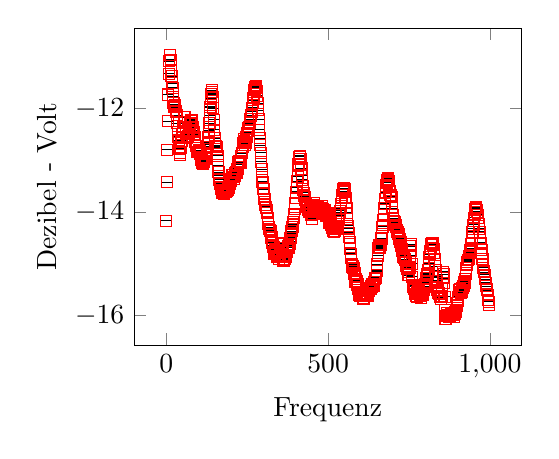
\begin{tikzpicture}
		\pgfplotsset{width=6.5cm,compat=1.3,legend style={font=\footnotesize}}
		\begin{axis}[xlabel={Frequenz},ylabel={Dezibel - Volt},legend cell align=left,legend pos=north west]
		\addplot+[only marks,color=red,mark=square,error bars/.cd,x dir=both,x explicit,y dir=both,y explicit,error bar style={color=black}] table[x=X,y=Y,x error=xerror,y error=yerror,row sep=\\]{			X	Y	xerror	yerror	\\			0.0	-14.164919	0	0	\\			1.464844	-13.423461	0	0	\\			2.929687	-12.795189	0	0	\\			4.394531	-12.245261	0	0	\\			5.859375	-11.730946	0	0	\\			7.324219	-11.329506	0	0	\\			8.789062	-11.085836	0	0	\\			10.253906	-10.961078	0	0	\\			11.71875	-10.973411	0	0	\\			13.183594	-11.064258	0	0	\\			14.648437	-11.258652	0	0	\\			16.113281	-11.375012	0	0	\\			17.578125	-11.516236	0	0	\\			19.042969	-11.597615	0	0	\\			20.507812	-11.773958	0	0	\\			21.972656	-11.89112	0	0	\\			23.4375	-11.958305	0	0	\\			24.902344	-11.977169	0	0	\\			26.367187	-11.933453	0	0	\\			27.832031	-11.946653	0	0	\\			29.296875	-12.067268	0	0	\\			30.761719	-12.043032	0	0	\\			32.226562	-12.130557	0	0	\\			33.691406	-12.287193	0	0	\\			35.15625	-12.452247	0	0	\\			36.621094	-12.543868	0	0	\\			38.085937	-12.618053	0	0	\\			39.550781	-12.772086	0	0	\\			41.015625	-12.893981	0	0	\\			42.480469	-12.850435	0	0	\\			43.945312	-12.752557	0	0	\\			45.410156	-12.653793	0	0	\\			46.875	-12.621641	0	0	\\			48.339844	-12.543832	0	0	\\			49.804687	-12.496791	0	0	\\			51.269531	-12.436894	0	0	\\			52.734375	-12.362595	0	0	\\			54.199219	-12.259872	0	0	\\			55.664062	-12.163448	0	0	\\			57.128906	-12.168667	0	0	\\			58.59375	-12.270183	0	0	\\			60.058594	-12.374486	0	0	\\			61.523437	-12.471527	0	0	\\			62.988281	-12.556238	0	0	\\			64.453125	-12.559223	0	0	\\			65.917969	-12.538605	0	0	\\			67.382812	-12.537811	0	0	\\			68.847656	-12.462484	0	0	\\			70.3125	-12.460954	0	0	\\			71.777344	-12.368802	0	0	\\			73.242187	-12.301627	0	0	\\			74.707031	-12.284165	0	0	\\			76.171875	-12.233723	0	0	\\			77.636719	-12.215283	0	0	\\			79.101562	-12.245056	0	0	\\			80.566406	-12.35783	0	0	\\			82.03125	-12.370201	0	0	\\			83.496094	-12.41712	0	0	\\			84.960937	-12.449146	0	0	\\			86.425781	-12.496071	0	0	\\			87.890625	-12.546374	0	0	\\			89.355469	-12.652713	0	0	\\			90.820312	-12.725718	0	0	\\			92.285156	-12.726218	0	0	\\			93.75	-12.755596	0	0	\\			95.214844	-12.835961	0	0	\\			96.679687	-12.832034	0	0	\\			98.144531	-12.833287	0	0	\\			99.609375	-12.847665	0	0	\\			101.074219	-12.808451	0	0	\\			102.539062	-12.823208	0	0	\\			104.003906	-12.833791	0	0	\\			105.46875	-12.871948	0	0	\\			106.933594	-12.967018	0	0	\\			108.398437	-12.999821	0	0	\\			109.863281	-13.033468	0	0	\\			111.328125	-13.055743	0	0	\\			112.792969	-13.065415	0	0	\\			114.257812	-13.051182	0	0	\\			115.722656	-13.015323	0	0	\\			117.1875	-13.033619	0	0	\\			118.652344	-12.974896	0	0	\\			120.117187	-12.933172	0	0	\\			121.582031	-12.963765	0	0	\\			123.046875	-12.965085	0	0	\\			124.511719	-12.859611	0	0	\\			125.976562	-12.738025	0	0	\\			127.441406	-12.690433	0	0	\\			128.90625	-12.661973	0	0	\\			130.371094	-12.560732	0	0	\\			131.835937	-12.429006	0	0	\\			133.300781	-12.285832	0	0	\\			134.765625	-12.138548	0	0	\\			136.230469	-11.972467	0	0	\\			137.695312	-11.806641	0	0	\\			139.160156	-11.721522	0	0	\\			140.625	-11.647183	0	0	\\			142.089844	-11.678916	0	0	\\			143.554687	-11.786087	0	0	\\			145.019531	-11.993779	0	0	\\			146.484375	-12.214814	0	0	\\			147.949219	-12.413501	0	0	\\			149.414062	-12.572942	0	0	\\			150.878906	-12.66897	0	0	\\			152.34375	-12.722298	0	0	\\			153.808594	-12.731719	0	0	\\			155.273437	-12.746778	0	0	\\			156.738281	-12.780426	0	0	\\			158.203125	-12.911675	0	0	\\			159.667969	-13.095085	0	0	\\			161.132812	-13.229077	0	0	\\			162.597656	-13.296058	0	0	\\			164.0625	-13.37067	0	0	\\			165.527344	-13.432754	0	0	\\			166.992187	-13.455957	0	0	\\			168.457031	-13.516274	0	0	\\			169.921875	-13.543134	0	0	\\			171.386719	-13.59857	0	0	\\			172.851562	-13.619785	0	0	\\			174.316406	-13.623	0	0	\\			175.78125	-13.632694	0	0	\\			177.246094	-13.644167	0	0	\\			178.710937	-13.613107	0	0	\\			180.175781	-13.6084	0	0	\\			181.640625	-13.610685	0	0	\\			183.105469	-13.615313	0	0	\\			184.570312	-13.600286	0	0	\\			186.035156	-13.577838	0	0	\\			187.5	-13.594874	0	0	\\			188.964844	-13.566325	0	0	\\			190.429687	-13.546297	0	0	\\			191.894531	-13.537756	0	0	\\			193.359375	-13.521826	0	0	\\			194.824219	-13.499905	0	0	\\			196.289062	-13.458123	0	0	\\			197.753906	-13.422541	0	0	\\			199.21875	-13.38834	0	0	\\			200.683594	-13.372364	0	0	\\			202.148437	-13.3292	0	0	\\			203.613281	-13.289784	0	0	\\			205.078125	-13.278719	0	0	\\			206.542969	-13.292925	0	0	\\			208.007812	-13.330059	0	0	\\			209.472656	-13.353241	0	0	\\			210.9375	-13.299781	0	0	\\			212.402344	-13.24685	0	0	\\			213.867187	-13.249435	0	0	\\			215.332031	-13.230795	0	0	\\			216.796875	-13.233479	0	0	\\			218.261719	-13.247204	0	0	\\			219.726562	-13.160436	0	0	\\			221.191406	-13.073816	0	0	\\			222.65625	-13.038491	0	0	\\			224.121094	-13.022263	0	0	\\			225.585937	-13.026715	0	0	\\			227.050781	-13.024103	0	0	\\			228.515625	-13.043439	0	0	\\			229.980469	-13.050436	0	0	\\			231.445312	-12.918389	0	0	\\			232.910156	-12.858723	0	0	\\			234.375	-12.861137	0	0	\\			235.839844	-12.740974	0	0	\\			237.304687	-12.67296	0	0	\\			238.769531	-12.621315	0	0	\\			240.234375	-12.595089	0	0	\\			241.699219	-12.646465	0	0	\\			243.164062	-12.703273	0	0	\\			244.628906	-12.673192	0	0	\\			246.09375	-12.601189	0	0	\\			247.558594	-12.551348	0	0	\\			249.023437	-12.503134	0	0	\\			250.488281	-12.468332	0	0	\\			251.953125	-12.43925	0	0	\\			253.417969	-12.385239	0	0	\\			254.882812	-12.368733	0	0	\\			256.347656	-12.377916	0	0	\\			257.8125	-12.284425	0	0	\\			259.277344	-12.210097	0	0	\\			260.742187	-12.144817	0	0	\\			262.207031	-12.127846	0	0	\\			263.671875	-12.057526	0	0	\\			265.136719	-11.99061	0	0	\\			266.601562	-11.897866	0	0	\\			268.066406	-11.838762	0	0	\\			269.53125	-11.791543	0	0	\\			270.996094	-11.728372	0	0	\\			272.460937	-11.649819	0	0	\\			273.925781	-11.615564	0	0	\\			275.390625	-11.594229	0	0	\\			276.855469	-11.56865	0	0	\\			278.320312	-11.610882	0	0	\\			279.785156	-11.657624	0	0	\\			281.25	-11.752055	0	0	\\			282.714844	-11.898074	0	0	\\			284.179687	-12.034184	0	0	\\			285.644531	-12.206844	0	0	\\			287.109375	-12.410667	0	0	\\			288.574219	-12.573703	0	0	\\			290.039062	-12.709421	0	0	\\			291.503906	-12.852396	0	0	\\			292.96875	-13.02938	0	0	\\			294.433594	-13.173633	0	0	\\			295.898437	-13.316868	0	0	\\			297.363281	-13.410936	0	0	\\			298.828125	-13.438397	0	0	\\			300.292969	-13.555132	0	0	\\			301.757812	-13.639437	0	0	\\			303.222656	-13.739624	0	0	\\			304.6875	-13.802883	0	0	\\			306.152344	-13.854175	0	0	\\			307.617187	-13.895003	0	0	\\			309.082031	-13.912361	0	0	\\			310.546875	-13.970285	0	0	\\			312.011719	-14.019984	0	0	\\			313.476562	-14.105786	0	0	\\			314.941406	-14.218993	0	0	\\			316.40625	-14.289461	0	0	\\			317.871094	-14.331567	0	0	\\			319.335937	-14.36875	0	0	\\			320.800781	-14.350113	0	0	\\			322.265625	-14.372686	0	0	\\			323.730469	-14.438382	0	0	\\			325.195312	-14.490969	0	0	\\			326.660156	-14.549839	0	0	\\			328.125	-14.594446	0	0	\\			329.589844	-14.640019	0	0	\\			331.054687	-14.676335	0	0	\\			332.519531	-14.778669	0	0	\\			333.984375	-14.805493	0	0	\\			335.449219	-14.79087	0	0	\\			336.914062	-14.725665	0	0	\\			338.378906	-14.751975	0	0	\\			339.84375	-14.795754	0	0	\\			341.308594	-14.850716	0	0	\\			342.773437	-14.865397	0	0	\\			344.238281	-14.8571	0	0	\\			345.703125	-14.87169	0	0	\\			347.167969	-14.89667	0	0	\\			348.632812	-14.91024	0	0	\\			350.097656	-14.866378	0	0	\\			351.5625	-14.822433	0	0	\\			353.027344	-14.697795	0	0	\\			354.492187	-14.606772	0	0	\\			355.957031	-14.603702	0	0	\\			357.421875	-14.684673	0	0	\\			358.886719	-14.743253	0	0	\\			360.351562	-14.822318	0	0	\\			361.816406	-14.944231	0	0	\\			363.28125	-14.943737	0	0	\\			364.746094	-14.917809	0	0	\\			366.210937	-14.901368	0	0	\\			367.675781	-14.908925	0	0	\\			369.140625	-14.873556	0	0	\\			370.605469	-14.848899	0	0	\\			372.070312	-14.768765	0	0	\\			373.535156	-14.726537	0	0	\\			375.0	-14.675093	0	0	\\			376.464844	-14.650801	0	0	\\			377.929687	-14.686325	0	0	\\			379.394531	-14.685237	0	0	\\			380.859375	-14.615952	0	0	\\			382.324219	-14.559062	0	0	\\			383.789062	-14.498126	0	0	\\			385.253906	-14.416506	0	0	\\			386.71875	-14.366651	0	0	\\			388.183594	-14.32364	0	0	\\			389.648437	-14.28517	0	0	\\			391.113281	-14.232634	0	0	\\			392.578125	-14.183866	0	0	\\			394.042969	-14.118793	0	0	\\			395.507812	-14.037436	0	0	\\			396.972656	-13.932197	0	0	\\			398.4375	-13.834754	0	0	\\			399.902344	-13.734258	0	0	\\			401.367187	-13.606951	0	0	\\			402.832031	-13.529068	0	0	\\			404.296875	-13.406461	0	0	\\			405.761719	-13.313633	0	0	\\			407.226562	-13.193941	0	0	\\			408.691406	-13.081338	0	0	\\			410.15625	-12.978435	0	0	\\			411.621094	-12.928817	0	0	\\			413.085937	-12.911148	0	0	\\			414.550781	-12.982399	0	0	\\			416.015625	-13.087531	0	0	\\			417.480469	-13.159897	0	0	\\			418.945312	-13.285913	0	0	\\			420.410156	-13.380708	0	0	\\			421.875	-13.491495	0	0	\\			423.339844	-13.561915	0	0	\\			424.804687	-13.624795	0	0	\\			426.269531	-13.680864	0	0	\\			427.734375	-13.702535	0	0	\\			429.199219	-13.760435	0	0	\\			430.664062	-13.820443	0	0	\\			432.128906	-13.889204	0	0	\\			433.59375	-13.873719	0	0	\\			435.058594	-13.878381	0	0	\\			436.523437	-13.901205	0	0	\\			437.988281	-13.962881	0	0	\\			439.453125	-13.952352	0	0	\\			440.917969	-13.956283	0	0	\\			442.382812	-13.997928	0	0	\\			443.847656	-13.96912	0	0	\\			445.3125	-13.92994	0	0	\\			446.777344	-13.958331	0	0	\\			448.242187	-14.054118	0	0	\\			449.707031	-14.129704	0	0	\\			451.171875	-14.13127	0	0	\\			452.636719	-14.034574	0	0	\\			454.101562	-13.872049	0	0	\\			455.566406	-13.83161	0	0	\\			457.03125	-13.867401	0	0	\\			458.496094	-13.948902	0	0	\\			459.960937	-13.964863	0	0	\\			461.425781	-13.951336	0	0	\\			462.890625	-13.930324	0	0	\\			464.355469	-13.90534	0	0	\\			465.820312	-13.886018	0	0	\\			467.285156	-13.894171	0	0	\\			468.75	-13.94336	0	0	\\			470.214844	-13.963021	0	0	\\			471.679687	-13.95184	0	0	\\			473.144531	-13.928432	0	0	\\			474.609375	-13.9436	0	0	\\			476.074219	-13.993018	0	0	\\			477.539062	-13.972168	0	0	\\			479.003906	-13.927769	0	0	\\			480.46875	-13.919959	0	0	\\			481.933594	-13.878176	0	0	\\			483.398437	-13.933921	0	0	\\			484.863281	-14.006589	0	0	\\			486.328125	-14.042313	0	0	\\			487.792969	-14.040604	0	0	\\			489.257812	-13.989789	0	0	\\			490.722656	-13.965893	0	0	\\			492.1875	-14.013036	0	0	\\			493.652344	-14.079173	0	0	\\			495.117187	-14.058938	0	0	\\			496.582031	-14.042616	0	0	\\			498.046875	-14.028798	0	0	\\			499.511719	-14.024168	0	0	\\			500.976562	-14.052991	0	0	\\			502.441406	-14.127777	0	0	\\			503.90625	-14.19908	0	0	\\			505.371094	-14.198299	0	0	\\			506.835937	-14.161339	0	0	\\			508.300781	-14.20069	0	0	\\			509.765625	-14.245741	0	0	\\			511.230469	-14.29948	0	0	\\			512.695312	-14.314418	0	0	\\			514.160156	-14.326632	0	0	\\			515.625	-14.368225	0	0	\\			517.089844	-14.382597	0	0	\\			518.554687	-14.365603	0	0	\\			520.019531	-14.356421	0	0	\\			521.484375	-14.327419	0	0	\\			522.949219	-14.297708	0	0	\\			524.414062	-14.319672	0	0	\\			525.878906	-14.271985	0	0	\\			527.34375	-14.297767	0	0	\\			528.808594	-14.296371	0	0	\\			530.273437	-14.235972	0	0	\\			531.738281	-14.193714	0	0	\\			533.203125	-14.160018	0	0	\\			534.667969	-14.063418	0	0	\\			536.132812	-14.012983	0	0	\\			537.597656	-13.971955	0	0	\\			539.0625	-13.922511	0	0	\\			540.527344	-13.837942	0	0	\\			541.992187	-13.733746	0	0	\\			543.457031	-13.672196	0	0	\\			544.921875	-13.599367	0	0	\\			546.386719	-13.564062	0	0	\\			547.851562	-13.570491	0	0	\\			549.316406	-13.536284	0	0	\\			550.78125	-13.550315	0	0	\\			552.246094	-13.615621	0	0	\\			553.710937	-13.725394	0	0	\\			555.175781	-13.813622	0	0	\\			556.640625	-13.912788	0	0	\\			558.105469	-14.011829	0	0	\\			559.570312	-14.127286	0	0	\\			561.035156	-14.261301	0	0	\\			562.5	-14.315667	0	0	\\			563.964844	-14.396433	0	0	\\			565.429687	-14.474202	0	0	\\			566.894531	-14.581289	0	0	\\			568.359375	-14.717159	0	0	\\			569.824219	-14.807933	0	0	\\			571.289062	-14.892911	0	0	\\			572.753906	-15.006119	0	0	\\			574.21875	-15.048167	0	0	\\			575.683594	-15.042924	0	0	\\			577.148437	-15.041481	0	0	\\			578.613281	-15.08111	0	0	\\			580.078125	-15.143414	0	0	\\			581.542969	-15.18491	0	0	\\			583.007812	-15.236629	0	0	\\			584.472656	-15.340579	0	0	\\			585.9375	-15.320202	0	0	\\			587.402344	-15.283716	0	0	\\			588.867187	-15.33496	0	0	\\			590.332031	-15.403665	0	0	\\			591.796875	-15.396138	0	0	\\			593.261719	-15.473009	0	0	\\			594.726562	-15.577273	0	0	\\			596.191406	-15.589229	0	0	\\			597.65625	-15.594326	0	0	\\			599.121094	-15.608212	0	0	\\			600.585937	-15.598532	0	0	\\			602.050781	-15.593256	0	0	\\			603.515625	-15.585614	0	0	\\			604.980469	-15.588118	0	0	\\			606.445312	-15.599592	0	0	\\			607.910156	-15.624149	0	0	\\			609.375	-15.677808	0	0	\\			610.839844	-15.662599	0	0	\\			612.304687	-15.615596	0	0	\\			613.769531	-15.574302	0	0	\\			615.234375	-15.564623	0	0	\\			616.699219	-15.577662	0	0	\\			618.164062	-15.561067	0	0	\\			619.628906	-15.59237	0	0	\\			621.09375	-15.608487	0	0	\\			622.558594	-15.610703	0	0	\\			624.023437	-15.575845	0	0	\\			625.488281	-15.513718	0	0	\\			626.953125	-15.487089	0	0	\\			628.417969	-15.489087	0	0	\\			629.882812	-15.456893	0	0	\\			631.347656	-15.488946	0	0	\\			632.8125	-15.476543	0	0	\\			634.277344	-15.43681	0	0	\\			635.742187	-15.407044	0	0	\\			637.207031	-15.379602	0	0	\\			638.671875	-15.398109	0	0	\\			640.136719	-15.419669	0	0	\\			641.601562	-15.415136	0	0	\\			643.066406	-15.343995	0	0	\\			644.53125	-15.283542	0	0	\\			645.996094	-15.281807	0	0	\\			647.460937	-15.270488	0	0	\\			648.925781	-15.27723	0	0	\\			650.390625	-15.137238	0	0	\\			651.855469	-15.003118	0	0	\\			653.320312	-14.836588	0	0	\\			654.785156	-14.691212	0	0	\\			656.25	-14.64075	0	0	\\			657.714844	-14.676334	0	0	\\			659.179687	-14.69786	0	0	\\			660.644531	-14.664032	0	0	\\			662.109375	-14.638811	0	0	\\			663.574219	-14.62925	0	0	\\			665.039062	-14.508993	0	0	\\			666.503906	-14.417335	0	0	\\			667.96875	-14.28374	0	0	\\			669.433594	-14.250508	0	0	\\			670.898437	-14.155068	0	0	\\			672.363281	-14.052734	0	0	\\			673.828125	-13.924634	0	0	\\			675.292969	-13.843582	0	0	\\			676.757812	-13.743922	0	0	\\			678.222656	-13.61503	0	0	\\			679.6875	-13.48748	0	0	\\			681.152344	-13.428747	0	0	\\			682.617187	-13.386767	0	0	\\			684.082031	-13.353966	0	0	\\			685.546875	-13.352208	0	0	\\			687.011719	-13.406701	0	0	\\			688.476562	-13.511123	0	0	\\			689.941406	-13.603035	0	0	\\			691.40625	-13.605581	0	0	\\			692.871094	-13.671252	0	0	\\			694.335937	-13.686642	0	0	\\			695.800781	-13.704159	0	0	\\			697.265625	-13.792957	0	0	\\			698.730469	-13.924118	0	0	\\			700.195312	-14.058591	0	0	\\			701.660156	-14.118098	0	0	\\			703.125	-14.168582	0	0	\\			704.589844	-14.186841	0	0	\\			706.054687	-14.197821	0	0	\\			707.519531	-14.246687	0	0	\\			708.984375	-14.259801	0	0	\\			710.449219	-14.287938	0	0	\\			711.914062	-14.34451	0	0	\\			713.378906	-14.375563	0	0	\\			714.84375	-14.377806	0	0	\\			716.308594	-14.381978	0	0	\\			717.773437	-14.420093	0	0	\\			719.238281	-14.470079	0	0	\\			720.703125	-14.513393	0	0	\\			722.167969	-14.559719	0	0	\\			723.632812	-14.574286	0	0	\\			725.097656	-14.586582	0	0	\\			726.5625	-14.648714	0	0	\\			728.027344	-14.710528	0	0	\\			729.492187	-14.757821	0	0	\\			730.957031	-14.832319	0	0	\\			732.421875	-14.854806	0	0	\\			733.886719	-14.877755	0	0	\\			735.351562	-14.88173	0	0	\\			736.816406	-14.906705	0	0	\\			738.28125	-14.920448	0	0	\\			739.746094	-14.976879	0	0	\\			741.210937	-15.04167	0	0	\\			742.675781	-15.093629	0	0	\\			744.140625	-15.068466	0	0	\\			745.605469	-15.088859	0	0	\\			747.070312	-15.156895	0	0	\\			748.535156	-15.207619	0	0	\\			750.0	-15.21554	0	0	\\			751.464844	-15.080055	0	0	\\			752.929687	-14.842349	0	0	\\			754.394531	-14.653203	0	0	\\			755.859375	-14.619496	0	0	\\			757.324219	-14.75139	0	0	\\			758.789062	-14.999748	0	0	\\			760.253906	-15.250898	0	0	\\			761.71875	-15.411389	0	0	\\			763.183594	-15.442572	0	0	\\			764.648437	-15.424639	0	0	\\			766.113281	-15.482852	0	0	\\			767.578125	-15.493778	0	0	\\			769.042969	-15.583499	0	0	\\			770.507812	-15.611173	0	0	\\			771.972656	-15.61113	0	0	\\			773.4375	-15.579691	0	0	\\			774.902344	-15.632984	0	0	\\			776.367187	-15.552239	0	0	\\			777.832031	-15.530195	0	0	\\			779.296875	-15.528133	0	0	\\			780.761719	-15.586636	0	0	\\			782.226562	-15.576339	0	0	\\			783.691406	-15.583306	0	0	\\			785.15625	-15.615468	0	0	\\			786.621094	-15.654258	0	0	\\			788.085937	-15.593427	0	0	\\			789.550781	-15.55961	0	0	\\			791.015625	-15.572397	0	0	\\			792.480469	-15.591817	0	0	\\			793.945312	-15.565172	0	0	\\			795.410156	-15.510333	0	0	\\			796.875	-15.454078	0	0	\\			798.339844	-15.432216	0	0	\\			799.804687	-15.439668	0	0	\\			801.269531	-15.393074	0	0	\\			802.734375	-15.349188	0	0	\\			804.199219	-15.271736	0	0	\\			805.664062	-15.224484	0	0	\\			807.128906	-15.193622	0	0	\\			808.59375	-15.169147	0	0	\\			810.058594	-15.118539	0	0	\\			811.523437	-15.001994	0	0	\\			812.988281	-14.873537	0	0	\\			814.453125	-14.811356	0	0	\\			815.917969	-14.758461	0	0	\\			817.382812	-14.687945	0	0	\\			818.847656	-14.611997	0	0	\\			820.3125	-14.610359	0	0	\\			821.777344	-14.599444	0	0	\\			823.242187	-14.60609	0	0	\\			824.707031	-14.630097	0	0	\\			826.171875	-14.704546	0	0	\\			827.636719	-14.790045	0	0	\\			829.101562	-14.899567	0	0	\\			830.566406	-15.047267	0	0	\\			832.03125	-15.12433	0	0	\\			833.496094	-15.251947	0	0	\\			834.960937	-15.324194	0	0	\\			836.425781	-15.440968	0	0	\\			837.890625	-15.50808	0	0	\\			839.355469	-15.529231	0	0	\\			840.820312	-15.559946	0	0	\\			842.285156	-15.562803	0	0	\\			843.75	-15.575571	0	0	\\			845.214844	-15.61322	0	0	\\			846.679687	-15.628035	0	0	\\			848.144531	-15.624088	0	0	\\			849.609375	-15.676543	0	0	\\			851.074219	-15.637401	0	0	\\			852.539062	-15.465779	0	0	\\			854.003906	-15.276128	0	0	\\			855.46875	-15.153145	0	0	\\			856.933594	-15.197567	0	0	\\			858.398437	-15.371425	0	0	\\			859.863281	-15.635518	0	0	\\			861.328125	-15.89092	0	0	\\			862.792969	-16.0572	0	0	\\			864.257812	-16.011749	0	0	\\			865.722656	-15.997319	0	0	\\			867.1875	-15.977797	0	0	\\			868.652344	-15.953806	0	0	\\			870.117187	-15.985253	0	0	\\			871.582031	-15.978298	0	0	\\			873.046875	-16.031499	0	0	\\			874.511719	-16.009132	0	0	\\			875.976562	-16.00344	0	0	\\			877.441406	-16.01737	0	0	\\			878.90625	-15.959695	0	0	\\			880.371094	-15.939553	0	0	\\			881.835937	-15.960404	0	0	\\			883.300781	-15.980143	0	0	\\			884.765625	-15.976547	0	0	\\			886.230469	-15.964225	0	0	\\			887.695312	-16.028316	0	0	\\			889.160156	-15.987929	0	0	\\			890.625	-15.973478	0	0	\\			892.089844	-15.946158	0	0	\\			893.554687	-15.925603	0	0	\\			895.019531	-15.905794	0	0	\\			896.484375	-15.884222	0	0	\\			897.949219	-15.802191	0	0	\\			899.414062	-15.746722	0	0	\\			900.878906	-15.704599	0	0	\\			902.34375	-15.635251	0	0	\\			903.808594	-15.543485	0	0	\\			905.273437	-15.50399	0	0	\\			906.738281	-15.490819	0	0	\\			908.203125	-15.501112	0	0	\\			909.667969	-15.534743	0	0	\\			911.132812	-15.554223	0	0	\\			912.597656	-15.53789	0	0	\\			914.0625	-15.513728	0	0	\\			915.527344	-15.458383	0	0	\\			916.992187	-15.420981	0	0	\\			918.457031	-15.423178	0	0	\\			919.921875	-15.359825	0	0	\\			921.386719	-15.375223	0	0	\\			922.851562	-15.334644	0	0	\\			924.316406	-15.283337	0	0	\\			925.78125	-15.183854	0	0	\\			927.246094	-15.076307	0	0	\\			928.710937	-15.009317	0	0	\\			930.175781	-14.959847	0	0	\\			931.640625	-14.924248	0	0	\\			933.105469	-14.926521	0	0	\\			934.570312	-14.903872	0	0	\\			936.035156	-14.857246	0	0	\\			937.5	-14.778797	0	0	\\			938.964844	-14.729149	0	0	\\			940.429687	-14.741328	0	0	\\			941.894531	-14.697752	0	0	\\			943.359375	-14.616516	0	0	\\			944.824219	-14.498216	0	0	\\			946.289062	-14.384429	0	0	\\			947.753906	-14.316985	0	0	\\			949.21875	-14.244903	0	0	\\			950.683594	-14.165881	0	0	\\			952.148437	-14.109733	0	0	\\			953.613281	-14.059122	0	0	\\			955.078125	-13.939126	0	0	\\			956.542969	-13.897605	0	0	\\			958.007812	-13.911283	0	0	\\			959.472656	-13.957403	0	0	\\			960.9375	-13.994261	0	0	\\			962.402344	-14.049435	0	0	\\			963.867187	-14.115018	0	0	\\			965.332031	-14.221789	0	0	\\			966.796875	-14.322146	0	0	\\			968.261719	-14.383764	0	0	\\			969.726562	-14.495925	0	0	\\			971.191406	-14.589643	0	0	\\			972.65625	-14.620464	0	0	\\			974.121094	-14.724989	0	0	\\			975.585937	-14.797496	0	0	\\			977.050781	-14.896906	0	0	\\			978.515625	-15.02687	0	0	\\			979.980469	-15.071075	0	0	\\			981.445312	-15.132175	0	0	\\			982.910156	-15.159737	0	0	\\			984.375	-15.207652	0	0	\\			985.839844	-15.29338	0	0	\\			987.304687	-15.360249	0	0	\\			988.769531	-15.429519	0	0	\\			990.234375	-15.494858	0	0	\\			991.699219	-15.505591	0	0	\\			993.164062	-15.596383	0	0	\\			994.628906	-15.688907	0	0	\\			996.09375	-15.733156	0	0	\\			997.558594	-15.795795	0	0	\\		};		% \addlegendentry{Messpunkte Datensatz 0}
		\end{axis}
		\end{tikzpicture}	\caption{Umgebung}
	\label{fig:Umgebungsmessung}\end{figure}

        \subsubsection*{15 degrees}
            \begin{table}[H]
	\centering
	\begin{tabular}{cccccc}
		$\nu$ & c & C(c) & $\kappa$ & f\\
		\hline
		0.0 & 10.0(50) & 20.0(20) & 19.91(199) & 0.01(00) & -2.01(-02)	\\
		1.0 & 137.0(50) & 137.0(137) & 136.83(1368) & 0.33(003) & -2.99(-03)	\\
		2.0 & 267.0(50) & 178.0(178) & 177.84(1778) & 0.56(006) & -4.54(-045)	\\
		3.0 & 399.0(50) & 199.5(1995) & 199.35(1994) & 0.7(007) & -6.72(-067)	\\
		4.0 & 532.0(50) & 212.8(2128) & 212.67(2127) & 0.8(008) & -9.95(-099)	\\
		5.0 & 663.0(50) & 221.0(221) & 220.88(2209) & 0.86(009) & -14.47(-145)	\\
		6.0 & 797.0(50) & 227.71(2277) & 227.6(2276) & 0.91(009) & -23.5(-235)	\\
		7.0 & 931.0(50) & 232.75(2328) & 232.64(2326) & 0.96(01) & -45.27(-453)	\\
		0.0(00) & 467.0(177) & 178.6(674) & 178.46(674) & 0.64(003) & -13.68(068)	\\
	\end{tabular}
\end{table}
            \begin{table}[H]
	\centering
	\begin{tabular}{cccccc}
		$\nu$ & c & C(c) & $\kappa$ & f\\
		\hline
		0.0 & 10.0(50) & 20.0(20) & 19.91(199) & 0.01(00) & -2.01(-02)	\\
		1.0 & 137.0(50) & 137.0(137) & 136.83(1368) & 0.33(003) & -2.99(-03)	\\
		2.0 & 267.0(50) & 178.0(178) & 177.84(1778) & 0.56(006) & -4.54(-045)	\\
		3.0 & 399.0(50) & 199.5(1995) & 199.35(1994) & 0.7(007) & -6.72(-067)	\\
		4.0 & 532.0(50) & 212.8(2128) & 212.67(2127) & 0.8(008) & -9.95(-099)	\\
		5.0 & 663.0(50) & 221.0(221) & 220.88(2209) & 0.86(009) & -14.47(-145)	\\
		6.0 & 797.0(50) & 227.71(2277) & 227.6(2276) & 0.91(009) & -23.5(-235)	\\
		7.0 & 931.0(50) & 232.75(2328) & 232.64(2326) & 0.96(01) & -45.27(-453)	\\
		0.0(00) & 467.0(177) & 178.6(674) & 178.46(674) & 0.64(003) & -13.68(068)	\\
	\end{tabular}
\end{table}

        \subsubsection*{10 degrees}
            \begin{table}[H]
	\centering
	\begin{tabular}{ccccc}
		c & C(c) & $\kappa$ & f\\
		\hline
		8 & 134 & 263 & 394 & 528 & 656 & 785 & 914	\\
		16.0 & 134.0 & 175.33333333333331 & 197.0 & 211.20000000000002 & 218.66666666666666 & 224.28571428571428 & 228.5	\\
		15.917637722755833 & 133.83145892641542 & 175.17592055945 & 196.85549879388316 & 211.06617713931504 & 218.54236297645 & 224.16916217553737 & 228.38995597589468	\\
		0.004516853879069811 & 0.31681495411163085 & 0.5424067117385064 & 0.6847444616907044 & 0.787016619889124 & 0.8436479300795946 & 0.8875632275605212 & 0.9212308747947763	\\
		-2.009074696837753 & -2.927464545713718 & -4.37069347673013 & -6.34405984023605 & -9.390404072650313 & -12.791643890727803 & -17.787774912131503 & -25.390659027750207	\\
	\end{tabular}
\end{table}
            \begin{table}[H]
	\centering
	\begin{tabular}{ccccc}
		c & C(c) & $\kappa$ & f\\
		\hline
		8 & 134 & 263 & 394 & 528 & 656 & 785 & 914	\\
		16.0 & 134.0 & 175.33333333333331 & 197.0 & 211.20000000000002 & 218.66666666666666 & 224.28571428571428 & 228.5	\\
		15.917637722755833 & 133.83145892641542 & 175.17592055945 & 196.85549879388316 & 211.06617713931504 & 218.54236297645 & 224.16916217553737 & 228.38995597589468	\\
		0.004516853879069811 & 0.31681495411163085 & 0.5424067117385064 & 0.6847444616907044 & 0.787016619889124 & 0.8436479300795946 & 0.8875632275605212 & 0.9212308747947763	\\
		-2.009074696837753 & -2.927464545713718 & -4.37069347673013 & -6.34405984023605 & -9.390404072650313 & -12.791643890727803 & -17.787774912131503 & -25.390659027750207	\\
	\end{tabular}
\end{table}

        \subsubsection*{4 degrees}
            \begin{table}[H]
	\centering
	\begin{tabular}{cccccc}
		n & $\nu$ & c & C(c) & $\kappa$ & f\\
		\hline
		0.0 & 8.0(50) & 16.0(16) & 15.92(159) & 0.0(00) & -2.01(-02)	\\
		1.0 & 134.0(50) & 134.0(134) & 133.83(1338) & 0.32(003) & -2.93(-029)	\\
		2.0 & 263.0(50) & 175.33(1753) & 175.18(1752) & 0.54(005) & -4.37(-044)	\\
		3.0 & 393.0(50) & 196.5(1965) & 196.36(1964) & 0.68(007) & -6.27(-063)	\\
		4.0 & 523.0(50) & 209.2(2092) & 209.07(2091) & 0.77(008) & -8.78(-088)	\\
		5.0 & 649.0(50) & 216.33(2163) & 216.21(2162) & 0.83(008) & -11.48(-115)	\\
		6.0 & 781.0(50) & 223.14(2231) & 223.03(223) & 0.88(009) & -16.47(-165)	\\
		7.0 & 909.0(50) & 227.25(2273) & 227.14(2271) & 0.91(009) & -22.52(-225)	\\
		0.0(00) & 457.5(177) & 174.72(661) & 174.59(66) & 0.62(002) & -9.35(041)	\\
	\end{tabular}
\end{table}
            \begin{table}[H]
	\centering
	\begin{tabular}{cccccc}
		n & $\nu$ & c & C(c) & $\kappa$ & f\\
		\hline
		0.0 & 8.0(50) & 16.0(16) & 15.92(159) & 0.0(00) & -2.01(-02)	\\
		1.0 & 134.0(50) & 134.0(134) & 133.83(1338) & 0.32(003) & -2.93(-029)	\\
		2.0 & 263.0(50) & 175.33(1753) & 175.18(1752) & 0.54(005) & -4.37(-044)	\\
		3.0 & 393.0(50) & 196.5(1965) & 196.36(1964) & 0.68(007) & -6.27(-063)	\\
		4.0 & 523.0(50) & 209.2(2092) & 209.07(2091) & 0.77(008) & -8.78(-088)	\\
		5.0 & 649.0(50) & 216.33(2163) & 216.21(2162) & 0.83(008) & -11.48(-115)	\\
		6.0 & 781.0(50) & 223.14(2231) & 223.03(223) & 0.88(009) & -16.47(-165)	\\
		7.0 & 909.0(50) & 227.25(2273) & 227.14(2271) & 0.91(009) & -22.52(-225)	\\
		0.0(00) & 457.5(177) & 174.72(661) & 174.59(66) & 0.62(002) & -9.35(041)	\\
	\end{tabular}
\end{table}
        
        \subsubsection*{0 degrees}
            \begin{table}[H]
	\centering
	\begin{tabular}{cccccc}
		n & $\nu$ & c & C(c) & $\kappa$ & f\\
		\hline
		0.0 & 10.6(50) & 21.2(212) & 21.11(211) & 0.01(00) & -2.02(-02)	\\
		1.0 & 133.0(50) & 133.0(133) & 132.83(1328) & 0.31(003) & -2.91(-029)	\\
		2.0 & 282.0(50) & 188.0(188) & 187.84(1878) & 0.62(006) & -5.31(-053)	\\
		3.0 & 390.0(50) & 195.0(195) & 194.86(1949) & 0.67(007) & -6.08(-061)	\\
		4.0 & 521.0(50) & 208.4(2084) & 208.27(2083) & 0.77(008) & -8.56(-086)	\\
		5.0 & 647.0(50) & 215.67(2157) & 215.54(2155) & 0.82(008) & -11.15(-112)	\\
		6.0 & 776.0(50) & 221.71(2217) & 221.6(2216) & 0.87(009) & -15.07(-151)	\\
		7.0 & 907.0(50) & 226.75(2268) & 226.64(2266) & 0.91(009) & -21.55(-215)	\\
		0.0(00) & 458.32(177) & 176.22(664) & 176.08(663) & 0.62(002) & -9.08(039)	\\
	\end{tabular}
\end{table}
            \begin{table}[H]
	\centering
	\begin{tabular}{cccccc}
		n & $\nu$ & c & C(c) & $\kappa$ & f\\
		\hline
		0.0 & 10.6(50) & 21.2(212) & 21.11(211) & 0.01(00) & -2.02(-02)	\\
		1.0 & 133.0(50) & 133.0(133) & 132.83(1328) & 0.31(003) & -2.91(-029)	\\
		2.0 & 282.0(50) & 188.0(188) & 187.84(1878) & 0.62(006) & -5.31(-053)	\\
		3.0 & 390.0(50) & 195.0(195) & 194.86(1949) & 0.67(007) & -6.08(-061)	\\
		4.0 & 521.0(50) & 208.4(2084) & 208.27(2083) & 0.77(008) & -8.56(-086)	\\
		5.0 & 647.0(50) & 215.67(2157) & 215.54(2155) & 0.82(008) & -11.15(-112)	\\
		6.0 & 776.0(50) & 221.71(2217) & 221.6(2216) & 0.87(009) & -15.07(-151)	\\
		7.0 & 907.0(50) & 226.75(2268) & 226.64(2266) & 0.91(009) & -21.55(-215)	\\
		0.0(00) & 458.32(177) & 176.22(664) & 176.08(663) & 0.62(002) & -9.08(039)	\\
	\end{tabular}
\end{table}

    \subsection*{Adiabatic coefficient and degrees of freedom development}
        \begin{figure}[H]
	\centering
	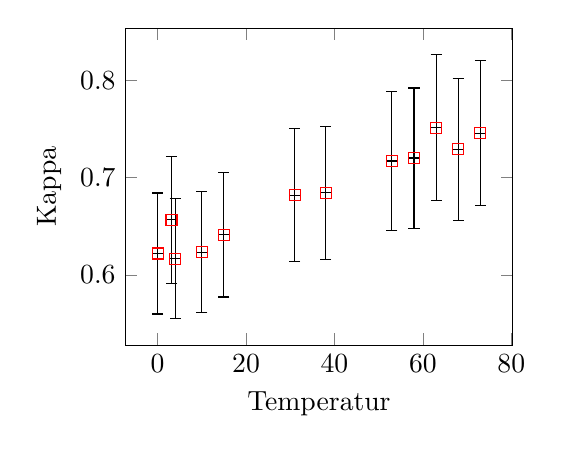
\begin{tikzpicture}
		\pgfplotsset{width=6.5cm,compat=1.3,legend style={font=\footnotesize}}
		\begin{axis}[xlabel={Temperatur},ylabel={Kappa},legend cell align=left,legend pos=north west]
		\addplot+[only marks,color=red,mark=square,error bars/.cd,x dir=both,x explicit,y dir=both,y explicit,error bar style={color=black}] table[x=X,y=Y,x error=xerror,y error=yerror,row sep=\\]{
			X	Y	xerror	yerror	\\
			3.141592653589793	0.6565661435410208	0	0.06565661435410208 	\\
			73	0.745651428687384	0	0.0745651428687384 	\\
			68	0.7291896973891191	0	0.07291896973891192 	\\
			63	0.7514142988993405	0	0.07514142988993405 	\\
			58	0.7202039843396486	0	0.07202039843396486 	\\
			53	0.7171452345550323	0	0.07171452345550323 	\\
			38	0.6845595922438421	0	0.06845595922438422 	\\
			31	0.682063770279751	0	0.06820637702797509 	\\
			15	0.6413677738717087	0	0.06413677738717087 	\\
			10	0.623492704217991	0	0.0623492704217991 	\\
			4	0.6165815992240085	0	0.06165815992240085 	\\
			0	0.622000108043746	0	0.062200010804374595 	\\
		};		% \addlegendentry{Messpunkte Datensatz 0}
		\end{axis}
		\end{tikzpicture}
	\caption{$\kappa(T)$}
	\label{fig:KappaTemperatur}
\end{figure}
        The above figure shows the correlation between the isentropic exponent and the temperature. Qualitatively, we can see that the isentropic exponent is higher when the temperature is higher. This expected, as $\kappa=\frac{f+2}{f}$ and we have more effective degrees of freedom for higher temperaturs: or vice versa, the colder a substance is, the less energy it has to active all its degrees of freedom.\\

        \noindent Additionally, the figure shown below plots the degrees of freedom over the temperature. The behaviour here is much more chaotic and even displays some negative degrees of freedom. This ist most likely due to a yet undiscovered calculation error.

        \begin{figure}[H]
	\centering
	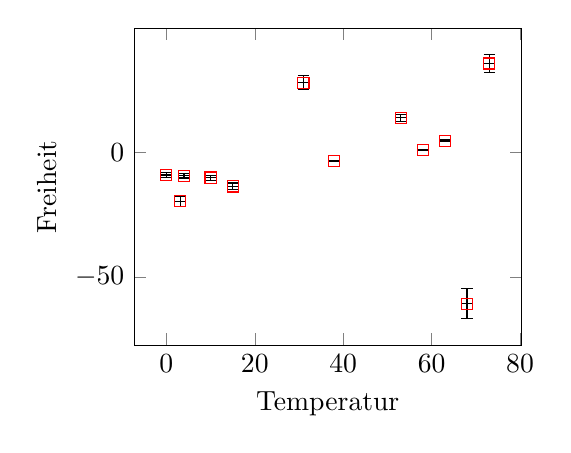
\begin{tikzpicture}
		\pgfplotsset{width=6.5cm,compat=1.3,legend style={font=\footnotesize}}
		\begin{axis}[xlabel={Temperatur},ylabel={Freiheit},legend cell align=left,legend pos=north west]
		\addplot+[only marks,color=red,mark=square,error bars/.cd,x dir=both,x explicit,y dir=both,y explicit,error bar style={color=black}] table[x=X,y=Y,x error=xerror,y error=yerror,row sep=\\]{
			X	Y	xerror	yerror	\\
			3.141592653589793	-19.587152221267605	0	-1.9587152221267605 (1/())	\\
			73	35.61118695932225	0	3.5611186959322247 (1/())	\\
			68	-60.65178959028931	0	-6.065178959028931 (1/())	\\
			63	4.697996134713314	0	0.4697996134713314 (1/())	\\
			58	0.8484052762734677	0	0.08484052762734678 (1/())	\\
			53	13.795175511942787	0	1.3795175511942788 (1/())	\\
			38	-3.4407061579130485	0	-0.3440706157913049 (1/())	\\
			31	27.950236316457676	0	2.7950236316457677 (1/())	\\
			15	-13.68049659008453	0	-1.3680496590084532 (1/())	\\
			10	-10.126471807847185	0	-1.0126471807847186 (1/())	\\
			4	-9.352740465879492	0	-0.9352740465879492 (1/())	\\
			0	-9.080536481984176	0	-0.9080536481984176 (1/())	\\
		};		% \addlegendentry{Messpunkte Datensatz 0}
		\end{axis}
		\end{tikzpicture}
	\caption{$f(T)$}
	\label{fig:FreiheitTemperatur}
\end{figure}
        
        
\end{document}